%%
% This is a sample document for writing a thesis which will be submitted
% to the Graduate School of Systems and Information Engineering.  The main
% purpose of this document is to reduce the author's trouble in making
% title.  Of course you can create your title page from scratch.  But your
% style must fulfill the requirements such as margins.
% 
%%
\documentclass[a4paper,11pt]{report}

%% [IMPORTANT] package for title generation (english version)
\usepackage{sie-en}
\usepackage{booktabs}
\usepackage{multirow}
\usepackage{graphicx}
\usepackage{algorithm}  
\usepackage{algorithmicx}  
\usepackage{algpseudocode}  
\usepackage{amsmath}
\usepackage{url}
\usepackage{xcolor}
\usepackage{enumitem}
\usepackage{listings}
\usepackage{amsfonts}

\lstset{language=[Objective]C, breakindent=40pt, breaklines, basicstyle=\scriptsize\ttfamily, numbers=left}

\algnewcommand{\LeftComment}[1]{\Statex \(\triangleright\) #1}

\renewcommand{\algorithmicrequire}{\textbf{Input:}}  
\renewcommand{\algorithmicensure}{\textbf{Output:}}  
\graphicspath{{figure/}}

\setcounter{tocdepth}{3}
\setcounter{page}{-1}

\setlength{\oddsidemargin}{0.1in}
\setlength{\evensidemargin}{0.1in} 
\setlength{\topmargin}{0in}
\setlength{\textwidth}{6in} 
%\setlength{\textheight}{10.1in}
\setlength{\parskip}{0em}
\setlength{\topsep}{0em}

\setlist[itemize,1]{label=$\bullet$}
\setlist[itemize,2]{label=$\diamond$}
\setlist[itemize,3]{label=$\times$}

%% title of thesis
%% DON'T PUT \\ AT THE END OF THE TITLE. IT CAUSES ERROR!!
\title{Developing Mobile Applications on Top of a Self-destruction System with Data Recovery}
%% name of author
\author{Meng Li}
%% name of advisor
\advisor{Yasushi Shinjo}

%% major and degree and date (chooose one)
%% [NOTICE] Month varies with majors.

\majorfield{Department of Computer Science} \degree{   } \yearandmonth{March 2018}


\begin{document}
		
\maketitle
\thispagestyle{empty}
\newpage

\thispagestyle{empty}
\vspace*{20pt plus 1fil}
%\parindent=1zw
\noindent
%%
%% Abstract
%%
\begin{center}
{\bf Abstract}
\vspace{5mm}
\end{center}
Conventional mobile applications are built based on a client-server modal and require central servers for storing shared data and processing confidential information.
If the central servers are accessed by an attacker, a curious administrator or a government, private information will be revealed because data is often stored on the central servers in the form of cleartext.
This thesis presents Grouper, a framework for developing mobile applications without trusted central servers.
With Grouper, it is easy to develop mobile applications on top of a self-destruction system with data recovery.
Grouper provides object synchronization among mobile devices.
It also uses a secret sharing scheme to create several shares from a marshalled object and uploads these shares to multiple untrusted servers. 
These untrusted servers construct a self-destruction system.
Uploaded shares will be deleted after a certain period of time.
Mobile devices exchange messages via untrusted servers based on the Grouper Message Protocol.
Grouper consists of a client framework and a Web service.
We have implemented client framework for iOS, macOS, tvOS and watchOS in Objective-C.
The Web service is implemented in Java and runs on multiple untrusted servers.
We have implemented two applications using Grouper: an iOS application named Account Book, and a benchmark application named Test.
We have evaluated the development efforts of applications using Grouper as well as the performance. 
Developing these applications demonstrates that Grouper requires little development effort to convert a standalone application to a data sharing application.
Experimental results prove that the performance of Grouper is satisfactory for mobile applications that are used among a small group of people.


%%%%%
\par
\vspace{0pt plus 1fil}
\newpage

\pagenumbering{roman} % I, II, III, IV 
\tableofcontents
\listoffigures
%\listoftables

\pagebreak \setcounter{page}{1}
\pagenumbering{arabic} % 1,2,3

\chapter{Introduction} \label{chapter:introduction}

People use mobile applications every day. 
When users use conventional mobile applications based on a client-server mode, users fully trust the central servers.
In fact, they are often unaware of their existence and simply rely on the functionality to be provided.
If the central servers are accessed by an attacker, a curious administrator or a government, private information will be revealed because data is often stored on the central servers in the form of cleartext.
In addition, users may lose their data when service providers shut their servers down.

To address the problem of using central servers, the proposals including Vanish\cite{geambasu2009vanish}, SafeVanish\cite{zeng2010safevanish}, SeDas\cite{zeng2012sedas} and CouldSky\cite{zeng2015cloudsky} constructed a data self-destruction system as their storage.
In these approaches, servers store encrypted data temporarily and delete it after a certain period of time.

These existing approaches have several problems.
First, they do not support data recovery when some nodes are unable to obtain data from shared storage.
Often, application developers have to deal with such cases on their own.
Second, these approaches do not provide support for developing mobile applications.

To address these problems, we develop such mobile applications on top of a self-destruction system with data recovery.
Concretely, we implement Grouper, a framework for developing mobile applications using such a self-destruction system\cite{li2017grouper}. 
Grouper provides object synchronization among mobile devices.
In Grouper, a sender node translates an updated object into shares using a secret sharing scheme and uploads these shares to untrusted servers. 
A receiver node downloads some of these shares and reconstructs the object.
The untrusted servers construct a self-destruction system, and delete these shares after a period of time.
Unlike existing approaches, Grouper supports data recovery when some nodes are unable to obtain shares from untrusted servers.
When a receiver node is unable to obtain shares, the Grouper framework automatically asks the sender to upload the missing shares again.
This ensures reliable data sharing among the devices of a group.
In addition, data can be recovered even if untrusted servers shut down because all devices of a group have the complete data set of this group.

Grouper consists of a client framework and a Web service.
We have implemented the client framework for iOS, macOS, tvOS and watchOS in Objective-C.
The Web service is implemented in Java and runs on multiple untrusted servers.
We used the Sync\cite{sync} framework in Grouper to synchronize objects among mobile nodes.
We have implemented two applications using Grouper: an iOS application named Account Book, and a benchmark application named Test.
These implementations demonstrate that Grouper makes it easy to develop mobile applications with data synchronization.
Experimental results prove that the performance of Grouper is satisfactory for mobile applications that are used among a small group of people.

The contributions of this paper are as follows.
First, we provide support for data recovery when some nodes are unable to obtain data from untrusted servers.
Grouper provides reliable data synchronization among nodes using a reliable multicast technique.
Second, we make it easier to develop mobile applications.
In fact, a developer can add data synchronization functions to stand alone applications with a few lines of code.

The rest of the paper is organized as follows.
We present related work in Chapter \ref{chapter:related_work}.
In Chapter \ref{chapter:threat_model}, we describe the threat model and some assumption in the Grouper framework.
In Chapter \ref{chapter:design}, we describe the layered design of Grouper, and the way to exchange messages among devices using the Grouper Message protocol.
In Chapter \ref{chapter:implementation}, we describe the three parts of implementation of Grouper: the client framework, the Web service and applications.
In Chapter \ref{chapter:evaluation}, we give the evaluation of Grouper using developement efforts and performance.
In Chapter \ref{chapter:conclusion}, we conclude the paper and show the future works.

\chapter{Related Work} \label{chapter:related_work}

In this chapter, we show related work. 
Most of them use data encryption that requires private key generation and distribution to protect user data, and do not support data recovery.

\section{Self-destruction Systems}

We show self-destruction systems which keep data on servers temporarily in the following subsections.

\subsection{Vanish}

Vanish\cite{geambasu2009vanish} is a self-destruction system that uses Distributed Hash Tables(DHTs) as the back-end storage.
Vanish encrypts a message with a new random key, threads the key to shares using a secret sharing scheme, stores these shares in a public DHT, and eliminates the key from the local storage.
The key in Vanish is removed after a certain period of time, and the encrypted message becomes permanently unreadable.
Vanish is implemented with OpenDHT\cite{rhea2005opendht} or VuzeDHT\cite{vuzedht} which is controlled by a single maintainer. 
Thus, it is not very secure against some Sybil attacks\cite{cholez2009evaluation, wolchok2010defeating}. 
In addition, the surviving time of the key in Vanish cannot be controlled by the applications for the user.

However, Vanish is not suitable for developing information sharing applications. 
Vanish is suitable for exchanging immutable messages, whereas our target applications need to modify objects repeatedly after other devices receive the object.


\subsection{SafeVanish and SeDas}

To address these issues in Vanish system, Zeng et al. proposed SafeVanish\cite{zeng2010safevanish} and SeDas\cite{zeng2012sedas}. 

SafeVanish prevents "hopping attacks"\cite{wolchok2010defeating}, which is one kind of the Sybil attacks\cite{cholez2009evaluation, wolchok2010defeating} by extending the length range of key shares to increase the attack cost substantially, and do some improvement on the Shamir's secret sharing algorithm implemented in the Vanish system.
The proposal of SafeVainish can only increase the cost of hoping attack, but cannot stop it.

Based on active storage framework like Oasis\cite{xie2011design}, SeDas proposes a distributed object-based storage system with self-destructing data function.
Concretely, it exploits active storage networks instead of P2P nodes to maintain a divided secret key. 
In SeDas, user can specify the key survival time of distribution key and use the settings of expanded interface to export the life cycle of a key, allowing the user to control the subjective life-cycle of private data.
The measurement and experimental security of SeDas nalysis sheds insight into the practicability of its approach.

Like Vanishe, SafeVanish and SeDas do not support the developent of information sharing applications.

\subsection{CloudSky}

Although, SeDas allows user to control the survival time of the key, it still cannot handle the cases that require the access control over the encrypted data including user grant and revocation.
By extending SeDas, Zeng's group proposed CloudSky\cite{zeng2015cloudsky}, a controllable data self-destruction system for untrusted cloud storage. 
CloudSky uses Attribute Bases Encryption (ABE) to implement the access control over the encrypted data, and allows the data owner to have user grant and revocation capabilities.
CouldSky deals with the untrusted cloud storage network in two ways including the data self-destruction and the use of Hash-based Message Authentication Code (HMAC) \cite{bellare1997hmac}, which ensures the data integrity.

CloudSky solves the problems regarding user controllability that exist in Vanish, but offline devices also cannot download messages after they have been removed from untrusted servers.
In Grouper, offline devices can download such messages by using confirm and resend messages.
A trusted authority is necessary in CloudSky to manage user profiles, whereas Grouper does not rely on any trusted authority.

\section{Using Untrusted Servers with Data Encryption}

We show systems that use data encryption in this section.
These systems encrypt user data and save the encrypted data in thee untrusted servers.

\subsection{Mylar}
Mylar\cite{popa2014building} stores encrypted data on an untrusted server and decrypts this data only in the browsers of users. 
Application developers of Mylar use its application program interface (API) to encrypt regular (non-encrypted) Web applications. 
Mylar uses its browser extension to decrypt data on the client-side. 
Mylar also supports keyword searching in Web applications by computing over encrypted data and JavaScript code verification in Web broswers.

Mylar enables client-side computation on data received from servers.
In addition, Mylar still requires a trusted identity provider (IDP).
Compared to Mylar, which uses a single untrusted server, Grouper takes advantages of the data redundancy provided by the secret sharing scheme by using multiple untrusted servers and does not require any trusted IDP.

\subsection{DepSky}

DepSky\cite{bessani2013depsky} is a system that keeps encrypted data in commercial storage services and performs application logic in other individual servers.
It implements the concept of \emph{Cloud-of-Clouds}.  
\emph{Cloud-of-Clouds} is the core concept in DepSky.
It represents that DepSky is a virtual storage, and its users invoke operations in several individual severs. 
Figure \ref{fig:depsky} shows the architecture of DepSky.
When a client wants to share data with another client, it generates several shares and uploads these shares to the application logic servers on the left side.
Application logic servers encrypt and save shares into commercial storage services on the right side via the APIs provided by the storage provider.
By using commercial storage services, DepSky improves the availability and confidentiality of private information.

However, commercial storage services may not supports temporary data storage like the self-destruction systems.
In Grouper, untrusted servers undertake the responsibility of temporary data storage and message delivery.
Mobile devices perform application logic.

\begin{figure}
	\centering
	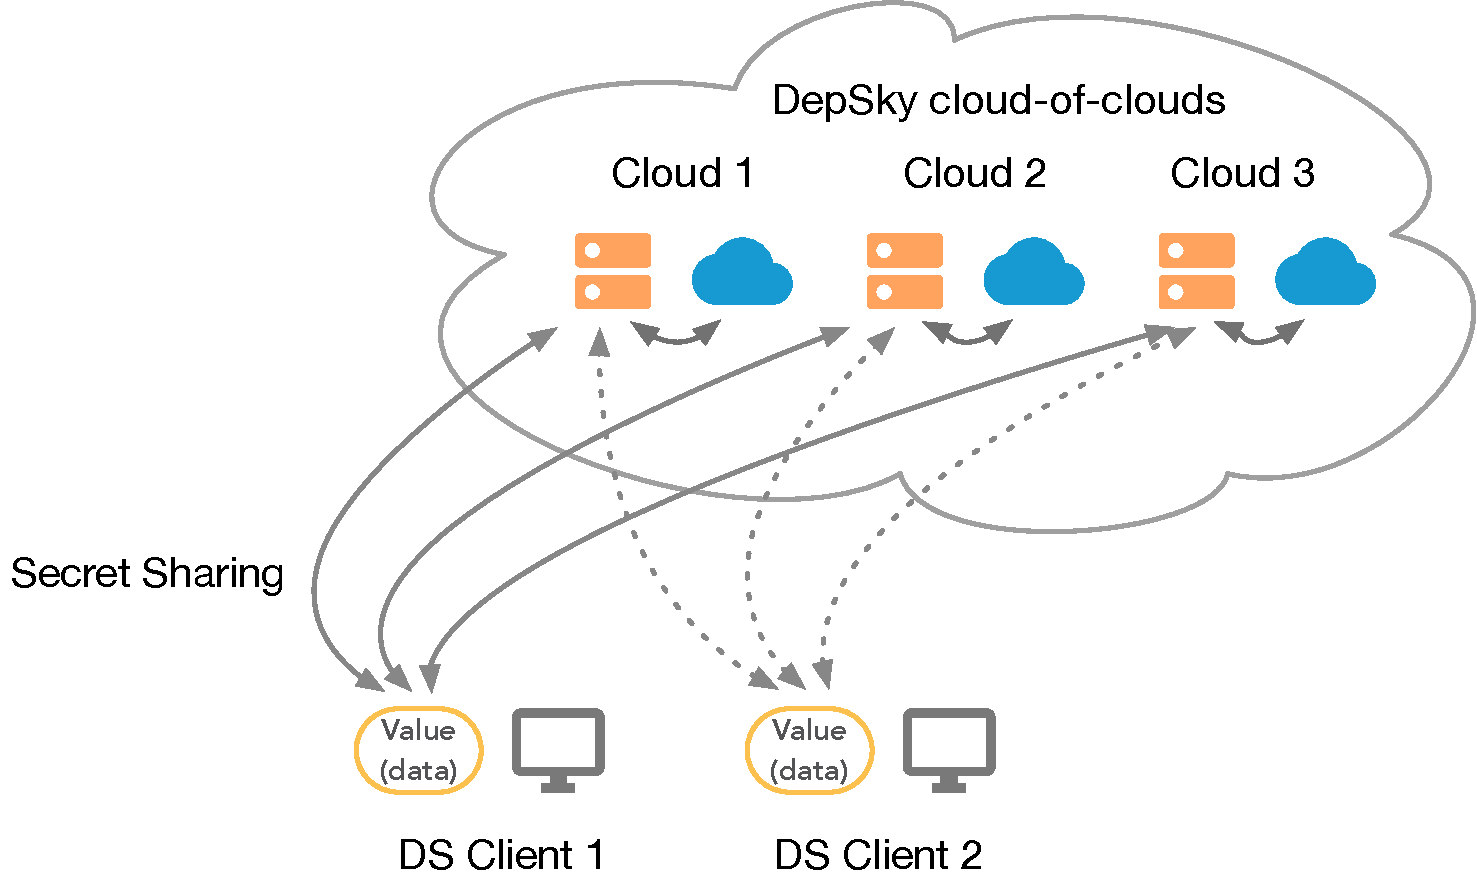
\includegraphics[scale=0.5]{depsky}
	\caption{Architecture of DepSky.}
	\label{fig:depsky}
\end{figure}

\subsection{SPORC}

SPORC\cite{feldman2010sporc} is designed for developing group collaboration applications using untrusted cloud resources.
In SPORC, a server observers only encrypted data and cannot deviate from correct execution without being detect.
From a conceptual distributed systems perspective, SPORC demonstrates the benefit if combing \emph{operational transformation} (OT)\cite{ellis1989concurrency} and \emph{fork* consistency}  protocols\cite{li2007beyond}.
To maintain synchronization among clients, SPORC uses OT, which allows each client to apply local updates optimistically.
To solve the problem that the server causes the views of two clients to diverge, SPROC uses fork* consistency protocol, which is a consistency model for interacting with an untrusted server.

In SPORC, synchronization should be done among online nodes, while Grouper allows synchronization among offline nodes.

\section{Peer-to-peer System}

In this secton, we shoe an application Sweets\cite{sweets} using peer-to-peer (P2P) technique. 
Sweets is a decentralized social networking service (SNS) application on Android devices that uses data synchronization with P2P connections among mobile devices. 
Sweets performs data synchronization not only between two online nodes directly but also via common friend nodes indirectly for offline nodes.
This indirect synchronization uses ABE to provide access control.
Consequently, Sweets provides data confidentiality and availability without permanently available centralized storage servers.
Sweets applys OpenID Connect\cite{openidconnect} to provide decentralized user authentication and implements a self-issued OpenID\cite{openid} provider that runs on users’ devices.
Sweets implements indirect replication via a hybrid cryptographic mechanism that combines ABE and AES encryption schemes. 
Taking the advantage of ABE, protected data can be hosted and relayed by users who have no permission to access it. 
In addition, by combining ABE and AES, Sweets can void expensive and repetitive ABE operations.

Both Grouper and Sweets provide a way to develop mobile application without central servers.
However, direct synchronization in Sweets can only be done when two devices are online at the same time. 
On the other hand, in Grouper, users can synchronize data from multiple untrusted servers, anytime.

\chapter{Threat Model} \label{chapter:threat_model}

In this chapter, we describe the assumptions and the threat model underlying the Grouper framework.

We target mobile applications that are used among a small group of people.
A group consists of a special member called \emph{the owner} and other members.
Each member has a mobile device.
Only the group owner can invite other members in a face-to-face manner.
In this group, each user creates a new object and shares it with other grouper members.
When an user receives a new object from another user, he/she can edit the content of the object or delete the object.
The modification or deletion also sepreads to the devices of other group members.

Our target applications supports the groups that have sensitive shared data.
Those groups must prevent access to shared data by other parties including server manager.

To implement such mobile applications, we assume the following assumptions in Grouper.

First, because we use servers, they are passive adversaries and can read all of the data but they do not actively attack.
Servers host Web services and perform device authentication.
Servers generate access keys for group members. 
When a device wants to get/put data from/to servers, the device sends a request with an access key.
In this paper, we do not address other types of attacks such as user tracking and metadata collection by servers. 
For example, servers can track users with IP addresses, and Grouper cannot hide social graphs against such tracking.

Second, data transportation between a device and an untrusted server is secure.
We can protect it using Transport Layer Security (TLS) or other encryption techniques.
Grouper focuses on the privacy of the data storage on servers rather than on data transportation.

Third, in an application, all group members are not malicious and their devices connect to each other securely at a face-to-face distance at the time of user invitation.
For example, group members working in an office know one another and are not malicious.
When the group owner invites new members, the owner authenticates group members in a face-to-face manner.
Note that after user invitation, devices communicate through servers and no secure, direct communication path is required.

Last, servers are isolated from one another and managed by independent providers.
We assume that providers of untrusted servers do not expose user data to other providers.
For example, a group owner can leverage the servers of Amazon, Google, and Microsoft, which are not supposed to expose user data to other cloud providers.

\chapter{Design} \label{chapter:design}

This chapter describes the design of the Grouper framework.

\section{Overview} \label{section:overview}

Our goal is to support the development of mobile applications that do not rely on trusted central servers.

To achieve this goal, we are developing the Grouper framework.
This framework provides the following functions:

\begin{itemize}[leftmargin=7mm]
	\setlength{\itemsep}{1pt}
	\setlength{\parskip}{0pt}
	\setlength{\parsep}{0pt}
	\item \textbf{Data Synchronization.} 
	If an user updates or deletes an object in his/her device, the mirrors of this object in other devices are updated or deleted.
	\item \textbf{Group management.} 
	A group owner can create a group and invite other members to his/her group.
\end{itemize}

For example, \emph{Account Book} is an iOS application developed using Grouper. 
In this application, a leader of a small company can create a group and invite employees to join the group. 
Then, the employees can record the income and expenditure of their company.
These income and expenditure records are represented as objects and shared among devices.
Anyone can edit and delete existing records in his/her device.

Grouper uses untrusted servers to exchange messages among mobile devices.
Untrusted servers construct a self-destruction system, and delete messages after a certain period of time.
We refer to this as the Time to Live (TTL).

Grouper uses Shamir's secret sharing scheme to protect messages from the providers of untrusted servers.
In this scheme, a member securely shares a secret with other members by generating $n$ shares using a cryptographic function\cite{smith2013layered}. 
At least $k$ or more shares can reconstruct the secret, but $k-1$ or fewer shares output nothing about the secret\cite{pang2005new}. 
We describe this scheme as a function ${f(k, n)}$, where $n$ is the number of shares, and $k$ is the threshold to combine shares. 

Grouper has the following advantages over conventional approaches using a self-destruction system.
First, it is easy for a developer to recover from message losses in untrusted servers, as demonstrated in Section \ref{section:reliable_message_delivery}.
Grouper performs retransmission when some mobile devices miss getting messages from untrusted servers.
Developers of mobile applications do not have to specify the lifetimes of messages.
Second, it is easy for a group owner to invite other members using a safe communication channel at a face-to-face distance, as discussed in Section \ref{section:group_management}.

\begin{figure}[t]
	\centering
	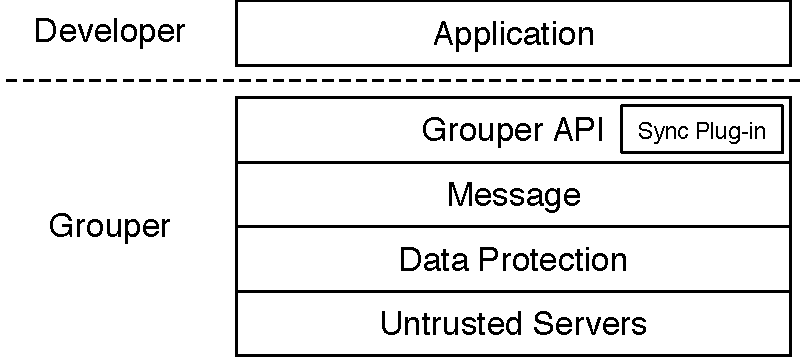
\includegraphics[scale=0.6]{architecture}
	\caption{Architecture of Grouper.}
	\label{fig:architecture}
\end{figure}

\section{Architecture} \label{section:architecture}

Figure \ref{fig:architecture} describes the architecture of the Grouper framework. 
Grouper consists of the following four layers and a plugin:

\begin{itemize}[leftmargin=7mm]
	\setlength{\itemsep}{1pt}
	\setlength{\parskip}{0pt}
	\setlength{\parsep}{0pt}
	\item \textbf{Grouper API.}
	A developer develops an application without data synchronization at first. 
	He/she adds the synchronization function to his/her application by using the API.
	\item \textbf{Synchronization Plugin.} 
	Grouper uses a third-party framework for data synchronization.
	This plugin marshalls an updated object in a local persistent store and the Grouper API layer passes the marshalled message to the lower message layer.
	When the Grouper API layer receives a message, this layer unmarshalls the message using the plugin, reconstructs the message, and puts the object included in the message into the persistent store.
	\item \textbf{Message.}
	This layer provides a messaging transportation service with multicasting capability among devices.
	The destination of a message is not only the node identifier (ID) of a single device, but also "*", which means it is delivered to all the other nodes.
	This layer does not ensure message delivery to other devices.
	\item \textbf{Data Protection.}
	Grouper protects user data by a secret sharing scheme in this layer.
	This layer divides a message into several shares, and uploads these shares to untrusted servers.
	When this layer downloads shares from untrusted servers, it recovers the original message using the secret sharing scheme.
	\item \textbf{Untrusted servers.}
	When a mobile device uploads a share to an untrusted server, this server receives it and stores it to a database.
	When a mobile device downloads a share from an untrusted server, this server retrieves it from the database and sends it into the device.
	An untrusted server performs device authentication using device keys.
\end{itemize}

The following sections describe the details of these layers from the top layer to the bottom layer.

\section{Grouper API} \label{section:grouper_api}

\begin{table}[t]
	\centering
	\caption{Client API of Grouper.}
	\label{table:grouper_api}
	\begin{tabular}{ll}
		\toprule
		\textbf{Method} & \textbf{Description} \\ 
		\midrule
		\begin{tabular}{@{}l@{}}
			$\textbf{setup}(appId, entities, dataStack)$
		\end{tabular} 
		 & 
		\begin{tabular}{@{}l@{}}
			An application invokes this method to initialize\\ Grouper with \emph{appId}, \emph{entities} and \emph{dataStack}. The\\ parameter \emph{appId} is the unique ID of an application.\\ The parameter \emph{entities} is an array which contains\\ the names of all entities used in this application.\\ The developer should pay attention to the order\\ of entity names in the array. If the entity A is referenced\\ by another entity B, A should be in front of B. The parameter\\ datastack is used by the synchronization plugin.
		\end{tabular}  \\ \hline
		$sender.\textbf{update}(object)$ & 
		\begin{tabular}{@{}l@{}}
			An application invokes this method after creating\\ a new object or modifying an existing object.\\ Grouper performs updates asynchronously\\ and sends an update message to other devices.
		\end{tabular} \\ \hline
		$sender.\textbf{delete}(object)$ & 
		\begin{tabular}{@{}l@{}}
			An application invokes this method when it wants\\ to delete an existing object. Grouper deletes the\\ object and removes it from the persistent store of\\ a device automatically, after sending a delete message\\ to other devices.
		\end{tabular} \\ \hline
		$receiver.\textbf{receive}(callback)$ & 
		\begin{tabular}{@{}l@{}}
			An application invokes this method to register the\\ callback function that is called after Grouper\\ processes the received messages and updates objects\\ according to the messages. The application\\ can use this callback function to update the user\\ screen. 
		\end{tabular} \\ \hline
		$sender.\textbf{confirm}()$ & 
		\begin{tabular}{@{}l@{}}
			An application needs to invoke this method\\ periodically or occasionally to send a confirm\\ message to other devices.
		\end{tabular} \\ 
		\bottomrule
	\end{tabular}
\end{table}

The Grouper framework provides object synchronization among mobile devices through a simple client API.

\subsection{Methods of Grouper API}

Table \ref{table:grouper_api} shows the client API of Grouper that is used to develop mobile applications.
An application initializes the framework by invoking the method $setup()$.
When the application needs to update an object in all devices, it invokes the method $sender.update()$.
When the application needs to delete an object in all devices, it invokes the method $sender.delete()$.
When the application needs to receive update notifications, it invokes the method $receiver.receive()$ with a callback function.
This callback function is called when another node updates an object and its local mirror has been updated.
The application can use this callback function to change the values that are shown on the user interface screen.
The method $sender.confirm()$ is used for realizing reliable messaging.
We will describe reliable messaging in Section \ref{section:reliable_message_delivery}.

\begin{table}[t]
	\centering
	\caption{API of the synchronization plugin.}
	\label{table:sync_plugin}
	\begin{tabular}{ll}
		\toprule
		\textbf{Method} & \textbf{Description} \\ 
		\midrule
		$marshall(o)$ & Marshalls the object o and returns the marshalled byte array. \\
		$updateRemote(b)$ & 
		\begin{tabular}{@{}l@{}}
			Unmarshalls the byte array $b$ to the object and puts the object into\\ the persistent store.
		\end{tabular} \\
		$deleteRemote(b)$ & Deletes the object of the object ID in the byte array $b$.\\ 
		\bottomrule
	\end{tabular}
\end{table}

These methods should be used after initializing the Grouper framework in the application's project.
We shoe the usage of these method in Section \ref{section:application}.

\subsection{Synchronization Plugin}

The Grouper API layer relies on the synchronization plugin.
As described in Table \ref{table:sync_plugin}, the synchronization plugin should provide the functions $marshall(o)$, $updateRemote(b)$ and $deleteRemote(b)$.
Grouper invokes these functions to obtain marshalled data from the persistent store, save unmarshalled data in the persistent store, and delete objects in the persistent store.

We have not implemented the synchronization plugin on our own, but we provide it as a pluggable module.
This is because there are many such synchronization modules that provide various features.
Additionally, application requirements may also vary.
Each application developer should choose a suitable module based on a consistency model and other requirements.

Because we implement our client framework in Objective-C, we currently user the Sync framework\cite{sync} to implement the data synchronization plugin.
The Sync framework marshalls objects into JavaScript Object Notation (JSON) strings and provides a consistency model where the newest version wins.

\section{Reliable Message Delivery}  \label{section:reliable_message_delivery}

Grouper implements reliable message delivery in the Grouper API layer over the self-destruction system.
In this section, we show an existing technique to solve the reliable message delivery problem called basic reliable multicasting at first.
Then we describe our own reliable message delivery protocol based on basic reliable multicasting technique.

\subsection{Basic Reliable Multicasting}

\begin{figure}[t]
	\centering
	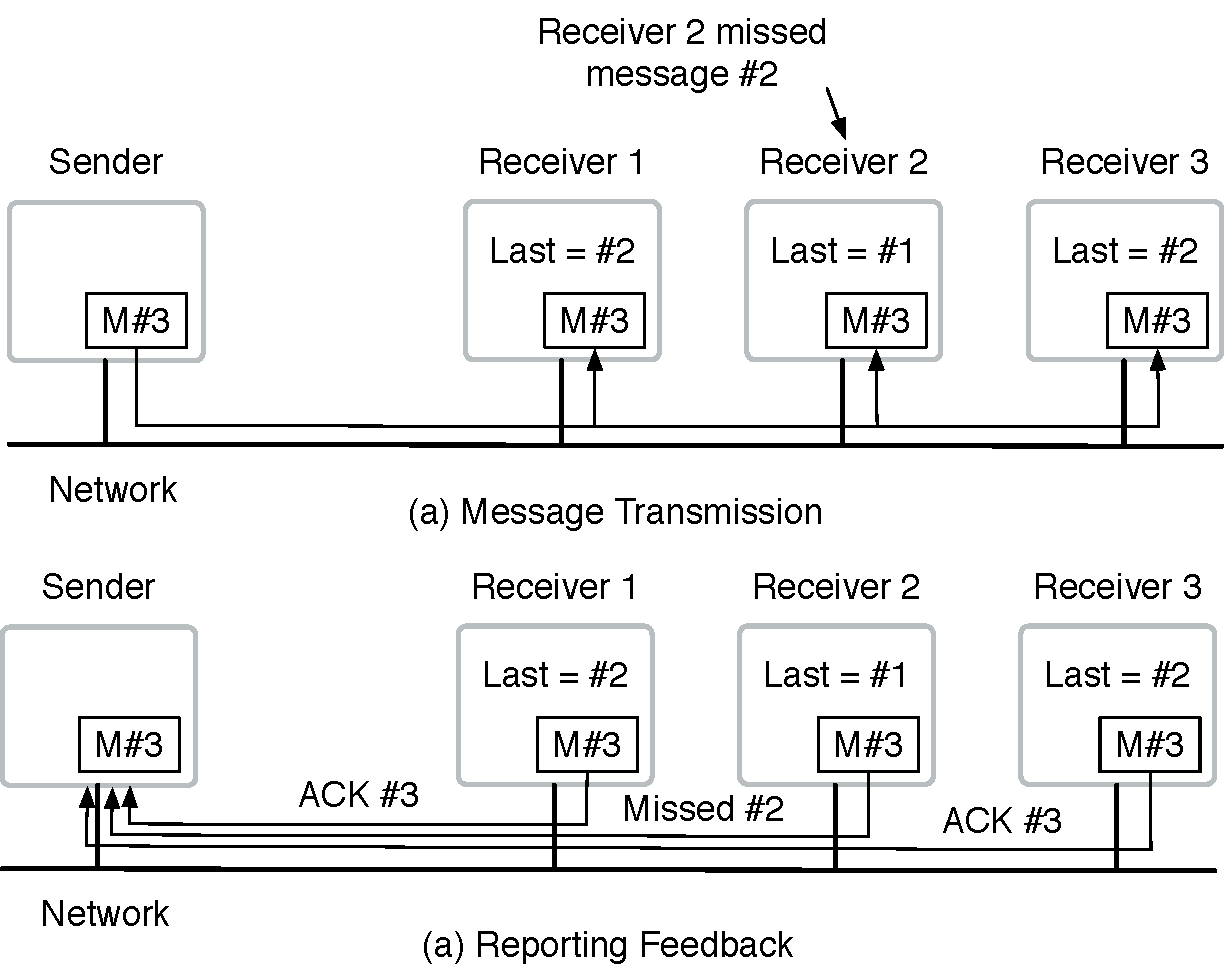
\includegraphics[scale=0.6]{reliable_multicasting}
	\caption{Basic reliable multicasting.}
	\label{fig:reliable_multicasting}
\end{figure}

Figure \ref{fig:reliable_multicasting} shows basic reliable multicasting technique in a text book\cite{tanenbaum2007distributed}.
In this reliable multicasting technique, each message has a sequence number for each sender a shown in Figure \ref{fig:reliable_multicasting}.
Each member keeps the newest sequence numbers for senders and detects missing messages.
If a member notices a missing message from a sender, the member asks the sender to resend the message.
For example, consider that a sender sends message No.3 to all other members using a multicast address.
When a member receives message No.3, the member compares the sequence number 3 with the newest sequence number of the sender.
If the newest sequence number of the sender is 1, this means the member missed message No.2.
The member asks the sender to resend message No.2 using a control message.
The sender will send message No.2 to the member who request it using a unicast address.

\subsection{Data Recovery on Self-destruction System}

This basic reliable multicasting technique works well for continuous media, such as video streaming in Internet communication.
However, it does not work well if receivers go offline often or for a long time, as our untrusted servers delete messages within a short time.
Therefore, the basic reliable multicasting technique is not suitable for data recovery on our self-destruction system.

To address this problem, we extend the basic reliable multicasting technique.
We use a special type of message that includes active sequence numbers.
Using these messages, a receiver can easily identify missing messages.
We call these type of messages \emph{confirm messages}.

\begin{figure}[t]
	\centering
	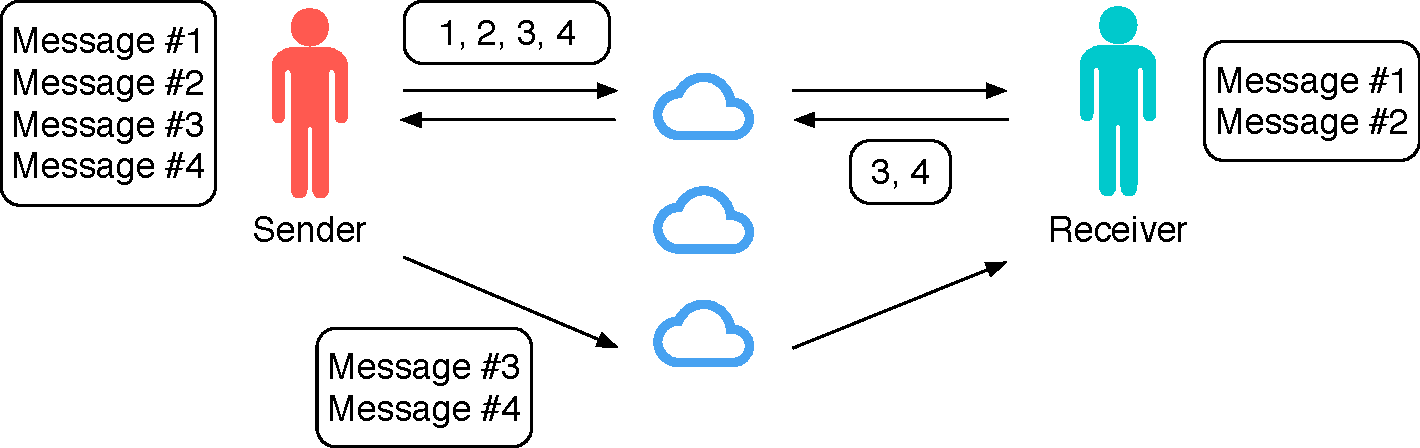
\includegraphics[scale=0.6]{reliable_sync}
	\caption{Implementing reliable messaging with continuous sequence numbers.}
	\label{fig:reliable_messaging}
\end{figure}

Figure \ref{fig:reliable_messaging} shows that the sender is sending five update messages, from No.1 to No.5, to the receiver.
The sender uploads two messages, No.1 and No.2, using a multicast address.
The receiver downloads these two messages and goes offline.
The servers delete these two messages.
The sender uploads the next three update messages, from No.3 to No.5, using a multicast address.
Then, the servers delete these three messages again.
The receiver comes online, but the receiver does not notice that these three messages are missing.

At this time, the sender sends a confirm message that includes the newest active sequence number, 5, as shown in Figure \ref{fig:reliable_messaging}.
The receiver receives this sequence number and compares it with the newest sequence number in the persistent store.
In Figure \ref{fig:reliable_messaging}, the receiver notices that update messages No.3, No.4, and No.5 are missing.
The receiver asks the sender to resend update messages No.3, No.4, and No.5 using a resend message.
The sender will again send update messages No.3, No. 4, and No.5 to the receiver using a unicast address.

This idea is inspired by the \emph{checkgroups} message of Usenet\cite{usenet}.
In Usenet, the list of active newsgroups is maintained with two basic messages: \emph{newgroup} and \emph{rmgroup}.
When a node receives a newgroup message, the node adds the newsgroup to the list.
When a node receives a rmgroup message, the node removes the newsgroup from the list.
However, these basic messages can be lost and the list can become obsolete.
Checkgroups messages supplement these basic messages.
A checkgroups message includes the list of all newsgroups in a newsgroup hierarchy.
A checkgroups message is distributed periodically or after some time after the basic messages are distributed.

\section{Data Protection}  \label{section:data_protection}

We design extend secret sharing scheme and data transportation flow based on this scheme to protect user data.

The data protection layer uses Shamir's secret sharing scheme $f(k, n)$ as shown in Section \ref{section:overview}.
In Grouper, we extend this scheme and design a new scheme $ f(k, n, s)$.
In our scheme, the parameters $k$ and $n$ are same as those in the scheme $f(k, n)$. 
The parameter $s$ represents the minimum number of untrusted servers when a sender uploads shares, where $k \leq s \leq n$.
Although a receiver is able to recover the original message from at least $k$ shares, we should also consider the scenario in which the server crashes. 
When a sender has $n$ shares, Grouper tries to upload these $n$ shares to all $n$ untrusted servers, at first. 
If the shares are uploaded to $s$ or more untrusted servers, we consider that this upload to be successful.
Otherwise, Grouper continues trying to upload these shares.

\begin{figure}[t]
	\centering
	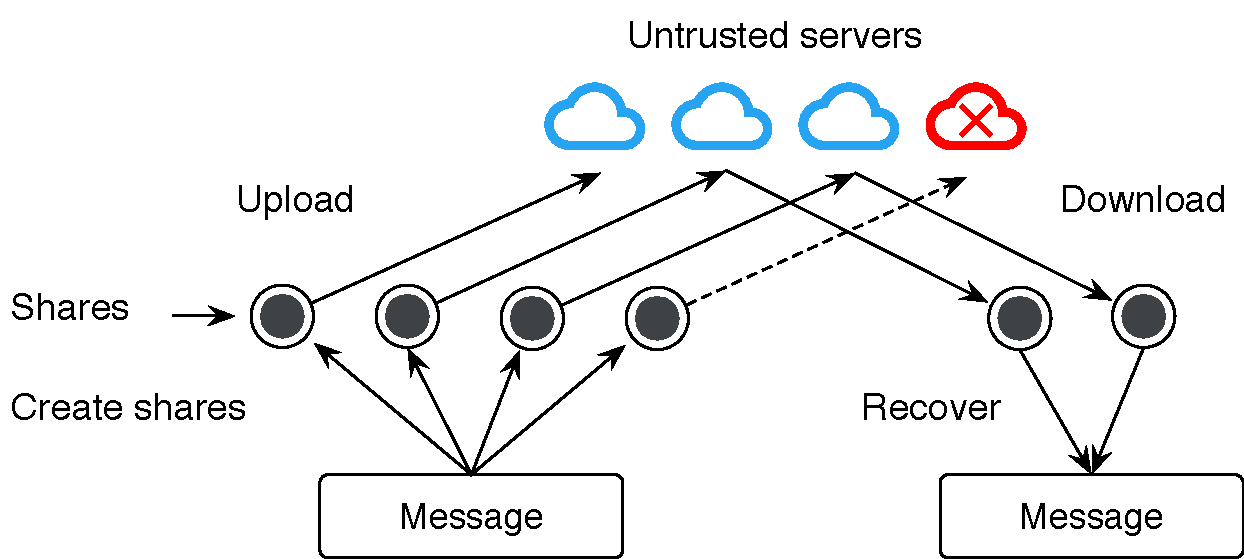
\includegraphics[scale=0.65]{transportation}
	\caption{Message transportation using the extended secret sharing scheme $f(2, 4, 3)$.}
	\label{fig:transportation}
\end{figure}

Figure \ref{fig:transportation} shows the message transportation from a device to another device using the extended secret sharing scheme $f(2, 4, 3)$.
In this figure, the message layer in a sender device is sending a message to the message layer in a receiver device.
At first, this layer calls the data protection layer and creates four shares, according to the secret sharing scheme.
Next, this layer uploads those shares to four untrusted servers.
In Figure \ref{fig:transportation}, although only the three untrusted servers on the left receives shares successfully, we regard this upload as successful, because we set $s = 3$ in the $f(k, n, s)$ scheme.
Finally, the message layer in the receiver device downloads two shares from the four untrusted servers and recovers the message by calling the data protection layer.

We can choose the parameter $s$ based on the following policies.

\begin{itemize}[leftmargin=7mm]
	\setlength{\itemsep}{1pt}
	\setlength{\parskip}{0pt}
	\setlength{\parsep}{0pt}
	\item \textbf{Sender first.} 
	An application sets $s$ close to $k$. 
	A sender receives a successful result earlier.
	When some servers are not available, it is more likely that a receiver will lose a message.
	\item \textbf{Receiver first.}
	An application sets $s$ close to $n$. 
	A sender must continue attempting to obtain a successful result.
	When some servers are not available, a receiver will be more likely to receive a message.
\end{itemize}

Compared to the traditional secret sharing scheme, the extended secret sharing scheme allows developers to tune the performance of uploading.

Compared with data encryption methods, the secret sharing scheme has the following advantages.
First, using a secret sharing scheme does not require key management, including generation and distribution.
Key generation and distribution usually need a central identity provider, which is against with the fully untrusted concept in Grouper.
Second, the secret sharing scheme ensures the data availability when a number of untrusted servers are not accessible.
For the $f(k, n, s)$ scheme in Grouper, a sender can complete uploading when at least $s$ untrusted servers are available, and a receiver can recover the object when at least $k$ untrusted servers are available.
Third, the secret sharing scheme reduces the risk of an attack because an attacker who can only access only $k-1$ or less untrusted servers cannot obtain any information.

\section{Grouper Message Protocol} \label{section:grouper_message_protocol}

The Grouper API layer sends and receives messages using our own protocol, the Grouper Message Protocol.
In this protocol, a message is a JSON string that contains a marshalled object and its attributes.

\subsection{Attributes of Grouper Message}

\begin{table}[t]
	\centering
	\caption{Attributes of the Grouper message.}
	\label{table:grouper_message_attributes}
	\begin{tabular}{lll}
		\toprule
		\textbf{Attribute} & \textbf{Explanation} \\ 
		\midrule
		type & Type of this message. \\
		content & A marshalled object or sequence numbers. \\
		sequence & Sequence number of the message. \\
		class & Class name of an object. \\
		objectId & ID of an object. \\
		receiverId & Node identifier of the receiver. \\
		senderId & Node identifier of the sender. \\
		email & Email address of the sender. \\
		name & Name of the sender. \\
		sentTime & Time the message is sent. \\
		\bottomrule
	\end{tabular}
\end{table}

Table \ref{table:grouper_message_attributes} shows the attributes in a Grouper message.
Figure \ref{fig:grouper_message} shows an example of an update message.
There are three important attributes:

\begin{itemize}[leftmargin=7mm]
	\setlength{\itemsep}{1pt}
	\setlength{\parskip}{0pt}
	\setlength{\parsep}{0pt}
	\item \textbf{Type.}
	This attribute refers to the message types.
	There are four types of messages: update messages, delete messages, confirm messages, and resend messages.
	An update message contains the marshalled objects of an application.
	A delete message contains the identifier of a deleted object.
	A confirm message contains the maximun sequence number of all update and delete messages created in a device.
	A resend message contains the sequence numbers of missing messages.
	We call update messages and delete messages \emph{normal messages}. 
	Both confirm messages and resend messages contain control information about a reliable multicast. 
	We call these messages \emph{control messages}.
	\item \textbf{Content.} 
	If the message is an update message, the content value contains the JSON string of a marshalled object.
	If the message is a delete message, the content value contains the objectId of an object.
	If the message is a confirm message, the content value contains the maximum sequence number of messages created in the device of the sender.
	If the message is a resend message, the content value contains the range of missing message sequence numbers.
	\item \textbf{Sequence.}
	This attribute refers to the sequence number of a message.
	When a sender sends a new normal message, the sender increments the sequence number and includes it in the new message.
	The sequence number of any control message is 0.
\end{itemize}

The receiverId attribute contains the addresses of destination devices.
An address is either a list of device IDs or "*", which signifies multicasting to all devices.

\begin{figure}
\caption{An update message.}
\label{fig:grouper_message}
\begin{lstlisting}[frame=none language=JSON] 
{
    "object" : "Test",
    "content" : "{\"content\":\"2017-09-2805:04:23+0000\",\"updator\":\"07DF1068-815C-4C70-B833-A6012B8BE846\",\"creator\":\"07DF1068-815C-4C70-B833-A6012B8BE846\",\"id\":\"A4ABC905-B6CE-4BA1-9224-F5AE7D0F0300\",\"update_at\":\"2017-09-28T14:04:23+09:00\",\"create_at\":\"2017-09-28T14:04:23+09:00\"}",
    "sender_id" : "07DF1068-815C-4C70-B833-A6012B8BE846",
    "receiver_id" : "*",
    "message_id" : "CEA7050B-CD14-4863-A127-A2C3FF74FBEC",
    "sequence" : 3,
    "email" : "test@test",
    "object_id" : "A4ABC905-B6CE-4BA1-9224-F5AE7D0F0300",
    "type" : "update",
    "name" : "test",
    "send_time" : 1506575063
}		
\end{lstlisting}
\end{figure}

Applications send update, delete and confirm messages through the Grouper API, and send resend messages after receiving confirm messages automatically.
When an application invokes the method $grouper.sender.update()$, the Grouper API layer sends an update message that contains the marshalled object to all devices.
When an application invokes the method $grouper.sender.delete()$, the Grouper API layer sends a delete message that contains the ID of the deleted object to all devices. 
When an application invokes the method $grouper.confirm()$, the Grouper API layer sends a confirm message to all devices. 
The confirm message includes the sequence numbers of objects that were recently created in the device.

The method $grouper.confirm()$ is invoked in the following situations:

\begin{itemize}[leftmargin=7mm]
	\setlength{\itemsep}{1pt}
	\setlength{\parskip}{0pt}
	\setlength{\parsep}{0pt}
	\item \textbf{Periodically.}
	For example, an application sends a confirm message once during the TTL.
	\item \textbf{When the device becomes online.} 
	Sometimes, a device is offline and cannot send a confirm message within the TTL.
	The device therefore sends a confirm message when the device becomes online.
\end{itemize}

\subsection{Algorithm to Handle Grouper Message}

Algorithm \ref{algorithm:receive_message} describes the handle process when the Grouper API layer receives a message.
For an update or delete message, Grouper invokes the method $sync.updateRemote()$ or $sync.deleteRemote()$ of the synchronization plugin to update the persistent store.
For a confirm message, the Grouper API layer copies the maximun sequence number from the message content.
Next, the Grouper API layer creates a resend message that contains the missing sequence numbers and sends it to the sender of the confirm message.
For resend messages, the Grouper API layer retrieves the sequence numbers from the resend message, finds the corresponding normal messages, and sends them to the sender of the resend message.

\begin{algorithm}[t]
	\caption{Message handling algorithm}\label{alg:euclid}
	\begin{algorithmic}[1]		
		\Procedure{onMessageReceived}{$msg,\ sender$}
		\LeftComment Check duplicate message.
		\State  $historyMsgs \gets getMsgsBySender(msg.sender)$
		\If{$msg \in historyMsgs$}
		\State \textbf{return}
		\EndIf
		\State $lastMsg \gets historyMsgs.last()$
		\State $historyMsgs.add(msg)$
		
		\LeftComment Basic reliable multicast.
		\If{$ msg.seq \neq  0 \ \&\& \ lastMsg.seq + 1 \neq  msg.seq$}
		\State $resendMsg \gets createResendMsg(lastMsg.seq\ +\ $ \\\hspace{2.7cm} $1,\ msg.seq)$
		
		\Comment Create a resend message with the minimum and maximum sequence number.
		\State $sendMsg(resendMsg,\ sender)$
		\EndIf
		
		\LeftComment Handle the message by its type.
		\If{$msg.type = "update"$}
		\State $sync.updateRemote(msg)$
		\ElsIf{$msg.type = "delete"$}
		\State $sync.deleteRemote(msg)$
		\ElsIf{$msg.type = "confirm"$}
		\State $maxSeq = getMaxSeqFrom(msg.content)$
		\State $resendMsg \gets createResendMsg(lastMsg.seq\ +\ $ \\\hspace{2.7cm}  $1,\ maxSeq)$
		\If{$resendMsg \neq null $}
		\State $sendMsg(resendMsg,\ sender)$
		\EndIf
		\ElsIf{$msg.type = "resend"$}
		\State $seqs \gets getSeqs(msg.content)$
		\For{$ seq \in seqs$}
		\State $missingMsg \gets getMsg(seq)$
		\State $sendMsg(missingMsg,\ sender)$
		\EndFor
		\EndIf
		\EndProcedure
	\end{algorithmic}
	\label{algorithm:receive_message}
\end{algorithm}

\section{Group Management}  \label{section:group_management}

To manage a group, Grouper provides the following two functions: group creation and member invitation.

\subsection{Group Creation}

A user can create a group, and the creator becomes the owner of the group.  
Before creating a group, the owner prepares his/her own user information (including his/her email address and name), multiple untrusted servers, a group ID, and a group name. 
Next, the owner initializes the group on all untrusted servers by submitting his/her node identifier and the TTL to multiple untrusted servers. 
The node identifier, which represents his/her device, is generated by Grouper randomly when the application is launched for the first time. 
On each untrusted server, the Web service initializes this new group and returns a master key including the highest privilege to the owner. 
The owner can add other members to an untrusted server using the master key.

\subsection{Member Invitation}

\begin{figure}
	\centering
	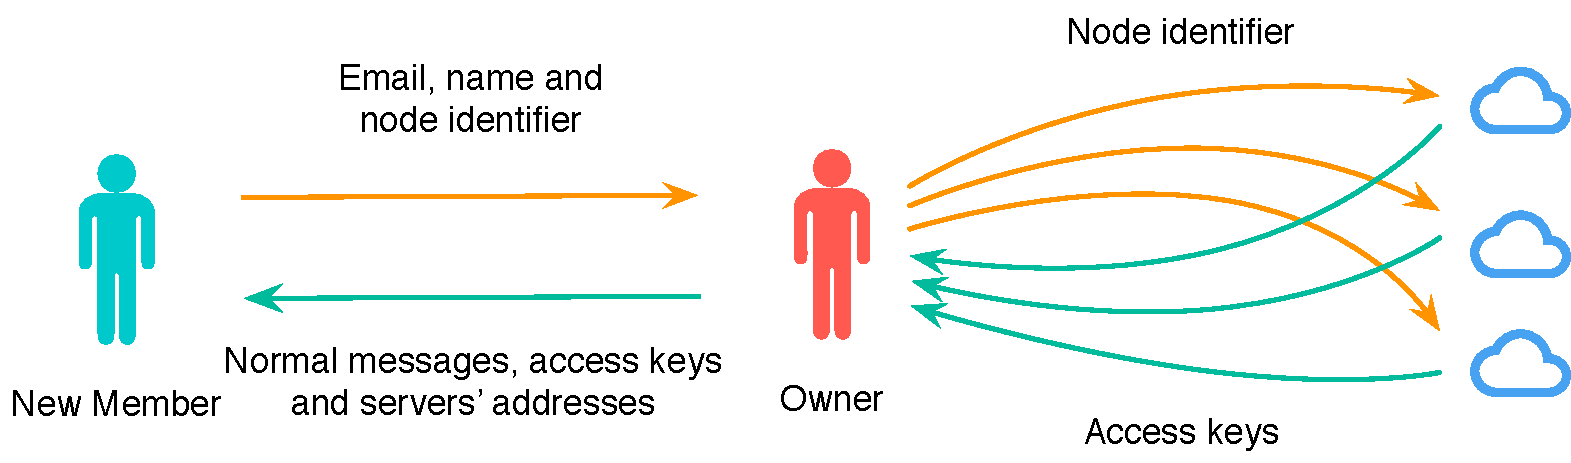
\includegraphics[scale=0.55]{add_member}
	\caption{Member invitation.}
	\label{fig:add_member}
\end{figure}

After creating a group, the owner can invite new members to his/her group as shown in Figure \ref{fig:add_member}. 
To join the group, a new member first prepares his/her user information. 
The owner invites the new member in a face-to-face manner, rather than using central servers. 
At this time, Grouper establishes a connection between the devices using a local safe communication channel like \emph{Multipeer Connectivity}\cite{mc}. 
First, the new member sends his/her user information and a node identifier to the owner. 
The owner saves the user information and node identifier to his/her device. 
Second, the owner registers the new member to the multiple untrusted servers by submitting the node identifier of the new member. 
Third, the untrusted servers return access keys for the new member to the owner. 
Last, the owner sends the access keys, the addresses of the untrusted servers, the list of existing members and all normal messages in his/her device to the new member.
After receiving them, the new member holds all data in the devie of group member and is able to access the untrusted servers with the keys.

\chapter{Implementation} \label{chapter:implementation}

Grouper consists of a client framework for developing mobile applications and a Web service running on multiple untrusted servers.
We describe the implementation of the implementation of the Web service in Section \ref{section:web_service}, the client framework in Section \ref{section:client_framework}, and demo applications in Section \ref{section:application}.

\section{Web Service} \label{section:web_service}

We have chosen to implement our own Web service rather than using commercial general cloud storage services like Amazon Simple Storage Service (S3), Google Cloud Storage, or Microsoft Azure Storage for the following reasons:

\begin{itemize}[leftmargin=7mm]
	\setlength{\itemsep}{1pt}
	\setlength{\parskip}{0pt}
	\setlength{\parsep}{0pt}
	\item The Web service must support on the Grouper Message protocol.
	\item The Web service must delete shares after a prescribed time.
\end{itemize}

\subsection{Application Servers, Databases and External Libraries and Frameworks} \label{subsection:dependencies_client}

Our Web service provides a RESTful API to clients.
It runs on a Tomcat server\cite{tomcat} that is an open-source implementation of the Java Servlet, JavaServer Pages, Java Expression Language, and Java WebSocket technologies.
Our Web service use the MySQL\cite{mysql} database as the backend storage.

We use the following frameworks in Java Enterprise Edition (Java EE) to implement our Web Service.

\begin{itemize}[leftmargin=7mm]
	\setlength{\itemsep}{1pt}
	\setlength{\parskip}{0pt}
	\setlength{\parsep}{0pt}
	\item 
	\textbf{Spring}\cite{spring}, a framework that provides a comprehensive programming and configuration model for modern Java-based enterprise applications.
	Grouper uses it for dependency injection, a technique whereby one object supplies the dependencies of another object, and managing containers in the Web project.
	\item 
	\textbf{Spring MVC}\cite{spring}, an original web framework built on the Servlet API and included in the Spring Framework.
	Spring MVC framework relies on the Spring framework.
	Grouper uses it to create our RESTful API.
	\item 
	\textbf{Hibernate}\cite{hibernate}, an open-source Java Object-Relational Mapping (ORM) framework.
	Hibernate provides generalized and automated solutions to common tasks associated with object life cycles and object graph management, including persistence. 
	Grouper uses it to save and operate objects in the Web service.
\end{itemize}

Our Web service has the following four layers.

\begin{itemize}[leftmargin=7mm]
	\setlength{\itemsep}{1pt}
	\setlength{\parskip}{0pt}
	\setlength{\parsep}{0pt}
	\item 
	\textbf{Domain Layer.}
	This layer is a collection of all entity objects.
	This layer creates a standardized and federated set of objects that are reused within different layers.
	\item 
	\textbf{Data Access Object (DAO) layer.}
	This layer is a collection of objects that provide abstract interface and implementation to access the MySQL database. 
	Each entity object corresponds to a DAO object.
	\item 
	\textbf{Service Layer.}
	This layer is a collection of objects that provide abstract interface and implementation of business logic.
	This layer invokes the methods of the DAO layer.
	\item 
	\textbf{Controller Layer.}
	The objects in this layer build the RESTful API for the client framework.
	This layer is responsible for user authentication with the access keys and invokes the methods of the service layer.
\end{itemize}

\subsection{Entity Design}

\begin{figure}
	\centering
	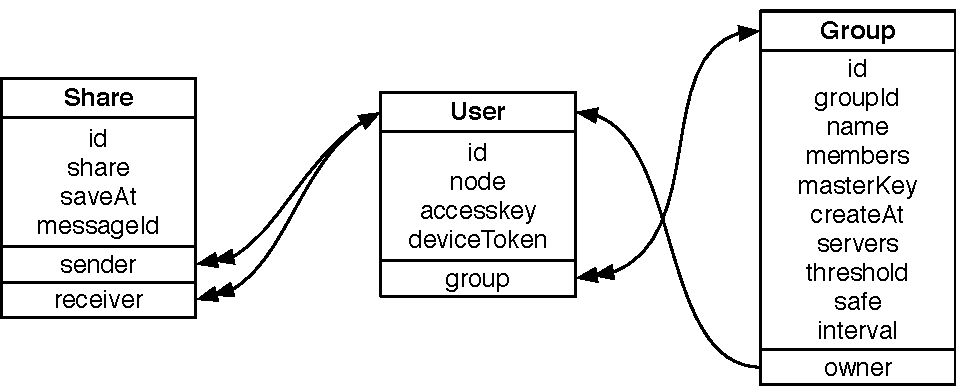
\includegraphics[scale=0.75]{server_entities}
	\caption{Entity relationship in the Web service of Grouper.}
	\label{fig:server_entities}
\end{figure}

\begin{table}[t]
	\centering
	\caption{Attributes of entities in the Web service of Grouper}
	\label{table:entity_attributes}
	\begin{tabular}{@{}lll@{}}
		\toprule
		\textbf{Entity} & \textbf{Attribute} & \textbf{Description} \\ \midrule
		\multirow{6}{*}{Share} & id & ID of the Share entity. \\
		& share & Share content uploaded from devices. \\ 
		& saveAt & Time the entity was saved. \\
		& messageId & Message ID of the share.\\
		& sender & User entity of the sender of the share. \\
		& receiver & User entity of the receiver of the share.  \\
		\hline
		\multirow{5}{*}{User} & id & ID of the User entity. \\
		& node & Device's unique node identifier of the user. \\
		& accessKey & Access key to upload and download shares of the user. \\
		& deviceToken & Device token for sending a remote notification. \\
		& group & Group of the user.  \\
		\hline
		\multirow{11}{*}{Group} & id & ID of the Group entity. \\
		& groupId & Unique group identifier created by the group owner. \\
		& name & Group name created by the group owner. \\
		& members & Number of group members. \\
		& masterKey & Master key for the group owner. \\
		& createAt & Time the entity was created. \\
		& servers & Number of servers, the parameter $n$ in the $f(k, n, s)$ scheme. \\
		& threshold & Threshold, the parameter $k$ in the $f(k, n, s)$ scheme. \\
		& safe & The parameter $s$ in the $f(k, n, s)$ scheme.  \\
		& TTL & Time to Live for the shares of this group.  \\
		& owner & User entity of the group owner. \\ 
		\bottomrule
	\end{tabular}
\end{table}

Our Web service includes three kinds of entities: the \emph{Group}, \emph{User}, and \emph{Share} entities.
Figure \ref{fig:server_entities} shows the relationship among these entities.
Table \ref{table:entity_attributes} shows the attributes of these entities.

Share entity saves the share content generate by a secret sharing scheme uploaded from the devices of group members.
To recover a message from multiple shares, we bind the message ID to the Share entity.
When a device downloads several shares from servers, Grouper tries to collect these shares by using the message ID and recover a message from the shares with the same message ID.
The sender attributes refers to an User entity, and indicates the uploading device.
The receiver attributes refers to an User entity, and indicates the devices that can download the share.
If the sender allows all devices in the group to receive the share, the receiver attribute of the entity is a $null$ value.

User entity saves the information of an user's device.
Each device has an unique node identifier of the UUID scheme.
Our untrusted server generates an access key for the user when the group owner register him/her in this server.
To receive a remote notification to the user, he/she should provide a device token to the notification pushing server.
The group attribute refers to a Group entity, and indicates which group the user belongs to.

Group entity saves the information of a group.
The group owner generates a unique group identifier, and gives a group name, to create a new group.
The number of group members is one when the owner creates the group.
When the group owner invites a new member to the group, the number of group members is incremented.
When the group is created, the server generates a master key and returns it to the group owner.
The group owner can update the attributes of the Group entity using this master key.
In addition, the group owner submits all parameters in the extended secret sharing scheme and the TTL.
The owner attribute refers to an User entity, and indicates the group owner.

\subsection{RESTful API}

The Web service of Grouper provides the following RESTful API for the client framework.

\begin{itemize}[leftmargin=7mm]
	\setlength{\itemsep}{1pt}
	\setlength{\parskip}{0pt}
	\setlength{\parsep}{0pt}
	\item 
	\textbf{group/register} (POST)
	\begin{itemize}
		\item Register a new group in an untrusted server.
		\item Parameters: group ID and group name.
		\item Return: master key for the group owner. 
	\end{itemize}
	\item 
	\textbf{group/info} (GET)
	\begin{itemize}
		\item Get information of a group.
		\item Header: master key of this group or access key of the group member.
		\item Return: all attributes of a Group entity. 
	\end{itemize}
	\item 
	\textbf{group/init} (POST)
	\begin{itemize}
		\item Initialize a group by submitting the parameters in the extended secret sharing scheme $f(k, n, s)$ and the TTL.
		\item Header: master key of this group.
		\item Parameters: $k$, $n$, $s$ and TTL.
		\item Return: success flag.
	\end{itemize}
	\item 
	\textbf{user/add} (POST)
	\begin{itemize}
		\item Add a new user in the untrusted server by the group owner.
		\item Header: master key of this group.
		\item Parameters: node identifier and the flag to indicate that this user is the owner or the common member.
		\item Return: access key for this new user.
	\end{itemize}
	\item 
	\textbf{user/state} (GET)
	\begin{itemize}
		\item Check server state.
		\item Header: access key of the group member.
		\item Return: server state.
	\end{itemize}
	\item 
	\textbf{user/deviceToken} (POST)
	\begin{itemize}
		\item Update the device token of the device by a group member.
		\item Header: access key of the group member.
		\item Parameters: access token from the remote notification pushing server.
		\item Return: success flag.
	\end{itemize}
	\item 
	\textbf{user/notify} (POST)
	\begin{itemize}
		\item Send a remote notification to a group member.
		\item Header: access key of the sender.
		\item Parameters: content of the remote notification, the node identifier of the notification receiver and the notification category.
		\item Return: success flag.
	\end{itemize}
	\item 
	\textbf{transfer/put} (POST)
	\begin{itemize}
		\item Upload a share to an untrusted server.
		\item Header: access key of the group member.
		\item Parameters: JSON array of which contains the shares, receivers and the message IDs.
		\item Return: the number of shares which are saved in the server successfully.
	\end{itemize}
	\item 
	\textbf{transfer/list} (GET)
	\begin{itemize}
		\item Get the list of share IDs for a group member.
		\item Header: access key of the group member.
		\item Return: share IDs that this group member has privilege to download.
	\end{itemize}
	\item 
	\textbf{transfer/get} (GET)
	\begin{itemize}
		\item Get the content of shares by the list of share IDs.
		\item Header: access key of the group member..
		\item Parameters: array of share IDs.
		\item Return: content of shares.
	\end{itemize}
	\item 
	\textbf{transfer/confirm} (POST)
	\begin{itemize}
		\item Confirm whether the shares are existed in an untrusted server. 
		\item Header: access key of the notification sender.
		\item Parameters: array of message IDs.
		\item Return: array of message IDs which are not existed in this untrusted server.
	\end{itemize}
\end{itemize}

All of these RESTful APIs authenticate the common group member or the group owner by submitting an access key or a master key in the request header.

\section{Client Framework} \label{section:client_framework}

\begin{figure}
	\centering
	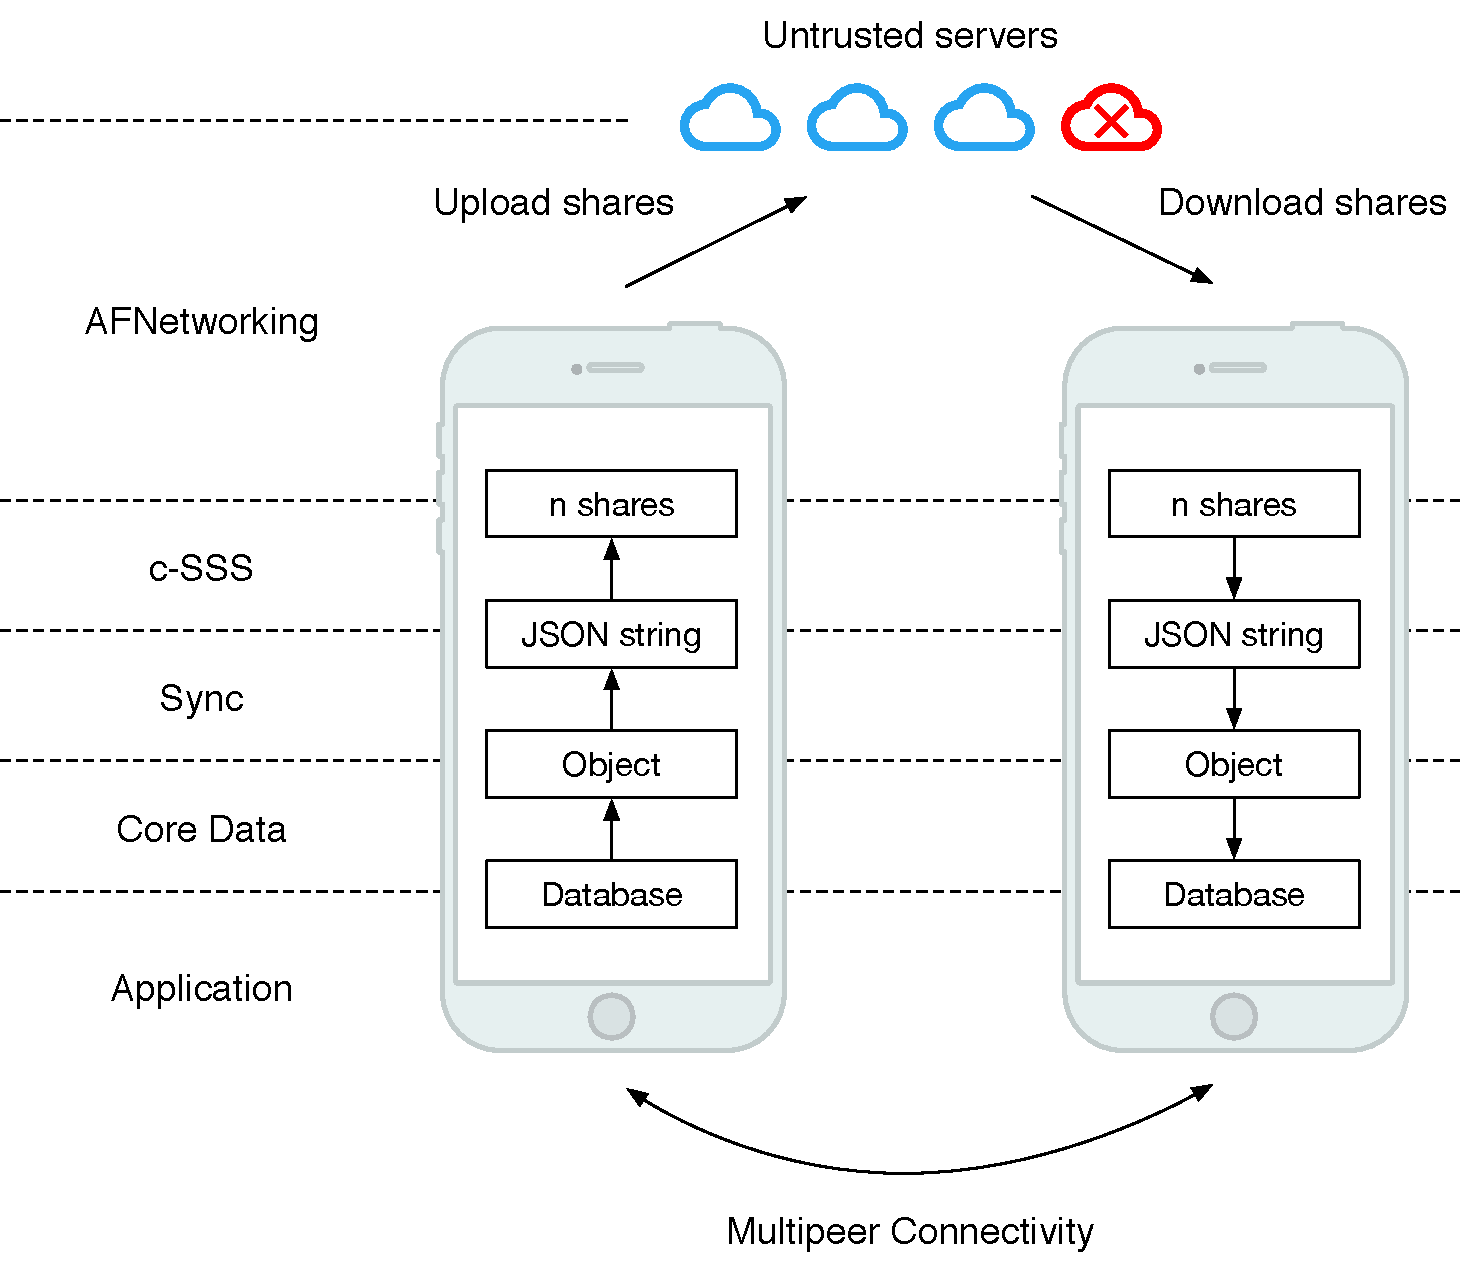
\includegraphics[scale=0.6]{frameworks}
	\caption{Frameworks in client framework of Grouper.}
	\label{fig:frameworks}
\end{figure}

This section describes how we implement the client framework.
Grouper's client framework is written in Objective-C, and its core layer supports developing applications on iOS, macOS, watchOS and tvOS.
Grouper supports the iOS graphical user interface (GUI) for group management, so that developers need not to implement it on the iOS platform.

In this section, we introduce the dependences of client framework in Subsection \ref{subsection:dependencies_client}.
We use singleton pattern to implement the manager classes in the client framework, to avoid multiple instances of a manager class.
These manager classes are listed from Subsection 

\subsection{Dependencies of Client Framework} \label{subsection:dependencies_client}

It makes use of the following frameworks in Figure \ref{fig:frameworks}.
The main functions of this frameworks are shown as following.

\begin{itemize}[leftmargin=7mm]
	\setlength{\itemsep}{1pt}
	\setlength{\parskip}{0pt}
	\setlength{\parsep}{0pt}
	\item 
	\textbf{Multipeer Connectivity}\cite{mc}, an official Peer-to-Peer communication framework provided by Apple. 
	Grouper uses it to transfer data between two devices in a face-to-face manner using a wireless LAN or Bluetooth network.
	With Multipeer Connectivity, a private connection can be established between two devices without Internet.
	\item 
	\textbf{Core Data}\cite{coredata}, an official ORM framework provided by Apple.
	Core Data provides generalized and automated solutions to common tasks associated with object life cycles and object graph management, including persistence. 
	Grouper uses it to manage model layer objects. 
	\item 
	\textbf{Sync}\cite{sync}, a lightweight Swift framework for data synchronization using Core Data.
	Sync uses the JSON string to synchronize managed objects of Core Data among devices.
	Sync provides a instance method $export()$ for the managed object to convert the it into a JSON string and an asynchronous method $sync(json, objectName, callback)$ for data stack to synchronize the JSON string into Core Data.
	Grouper currently uses it in the synchronization plugin.
	\item 
	\textbf{c-SSS}\cite{c-sss}, an implementation in the original C code of the secret sharing scheme. 
	It provide two main functions for generate shares and reconstructing them. The function $generate\_share\_strings(char * secret, int\ n, int\ k)$ can generate $n$ shares from the string secret with the threshold $k$. The function $extract_secret_from_share_strings(const char * shares)$ can recover the string after accessing to more than $k$ shares.
	\item 
	\textbf{AFNetworking}\cite{afnetworking}, a networking library in the Objective-C language. 
	Grouper uses it to invoke the RESTful API provided by our several Web services running on multiple untrusted servers. 
\end{itemize}

\subsection{Sender Manager} \label{subsection:sender_manager}

The class $SenderManager$ provides the methods to create and send the Grouper message as shown in Figure \ref{fig:sender_manager}.

In our persistent store, Core Data\cite{coredata}, the entities created by the application developers should synchronized to other devices.
We call an entity in Core Data which is needed to synchronize to other devices \emph{sync entity}.

\begin{figure}
\begin{lstlisting}[frame=none language=Objective-C] 
// Send an update message for a sync entity.
- (void)update:(NSManagedObject *)entity;

// Delete a sync entity and send a delete message.
- (void)delete:(NSManagedObject *)entity;

// Send confirm message;
- (void)confirm;

// Send resend message with a range to receiver.
- (void)resendWith:(int)min and:(int)max to:(NSString *)receiver;

// Send unsent messages.
- (void)unsent;

// Send existed messages.
- (void)sendExistedMessages:(NSArray *)messages;	
\end{lstlisting}
\caption{Instance methods of $SenderManager$.}
\label{fig:sender_manager}
\end{figure}

The method $- (void)update:$ creates an update messages with a JSON string generates from a sync entity. Then, invokes an instance method $- (void)sendMessages:$ to generate several shares from the normal messages and send the shares to multiple untrusted servers.

The method $- (void)delete:$ deletes a sync entity, creates a delete message with a JSON string which contains the object ID of this entity, and invokes the method $- (void)sendMessages:$, as same as the method $- (void)update:$ .

The method $- (void)confirm$ finds the maximum sequence number of normal messages in the local persistent store, creates a confirm message with a JSON string which contains the maximum sequence number, and invokes the method $- (void)sendMessages:$.

The method $- (void)resendWith:and:to:$ is used for sending a resend messages after receiving a confirm message.
It creates a resend message with a JSON string which contains the range of sequence number ( the minimum and maximum sequence number), and invokes the method $- (void)sendMessages:$.

Due to some network reasons, a device may send messages to untrusted servers using the method $- (void)sendMessages:$ unsuccessfully.
In these situations, the Grouper framework invokes the method $- (void)unsent$ to send the messages which are sent unsuccessfully.
The method $- (void)unsent$ finds those messages and sends them to untrusted servers again by invoking the method $- (void)sendMessages:$.

The method $- (void)sendExistedMessages:$ is used for resending normal messages after receiving a resend message.
It puts the normal message to a mutable array at first.
Before sending the normal messages, it confirms with the multiple untrusted servers at first.
If some of them have not been deleted in servers, those messages will be deleted from the mutable array.
At last, it sends the messages in the mutable array to servers by invoking the method $- (void)sendMessages:$.

The methods introduced above use a same important method $- (void)sendMessages:$, to generate shares and send to servers.
This method transfers the Grouper messages to a JSON strings at first.
Then, it invokes the function $generate\_share\_strings(char * secret, int\ n, int\ k)$ in c-SSS\cite{c-sss} to generate shares for each JSON string.
The shares are grouped by the address of the multiple untrusted server.
Next, it tries to upload these shares to the servers using the RESTful API \textbf{transfer/put}.
If the number of servers which are accessed successfully is more than $s$ in the extended secret sharing scheme $f(k, n, s)$, the Grouper framework regard this uploading successful.
Otherwise, the object IDs of these Grouper messages will be put into a queue called $unsentMessageIds$.
Grouper tries to send the Grouper messages recorded in $unsentMessageIds$, in the setup method, so that these messages can be sent with application launching.
At last, if the share uploading is successful, this method send a remote notification the messages' receiver.

Note that there may be too many messages to be sent at the same.
To improve the stability of the share uploading, the method $- (void)sendMessages:$ divide the messages to several parts.
For example, if there are 550 messages to be sent at the same, this method tries to send 100 messages everytime.

\subsection{Receiver Manager}

The class $ReceiverManager$ provides a instance method $- (void)receiveWithCompletion:$ to receive shares, recover messages and synchronize the content in the messages into the local persistent store.

This method does not download all shares from the multiple untrusted servers directly.
When the application invokes this method, it gets the array of share IDs from the servers using the RESTful API \textbf{transfer/list} at first.
Because Grouper saved the old share IDs in the local persistent store before, this method compares the new  share IDs from the servers with the old share IDs.
Then, this method removes those share IDs existed, and get the content of shares by submitting the share IDs which are not existed using the RESTful API \textbf{transfer/get}.
If the content of shares are received successfully, the share IDs will be saved into the local persistent store.
Next, this method tries to group the shares by message ID and recover the shares with a same message ID to a Grouper message.
At last, this method uses the Algorithm \ref{algorithm:receive_message} to handle the Grouper messages.
A callback block should be invoked after handling all messages successfully.

\subsection{GroupManager}

The class $GroupManager$ provides methods to create a new group, invite members to an existing group and send device token for remote notification to the untrusted servers.
Figure \ref{fig:group_manager} shows the main instance methods.

\begin{figure}
\begin{lstlisting}[frame=none language=Objective-C] 
// Save global user email and name.
- (void)saveCurrentUserWithEmail:(NSString *)email name:(NSString *)name;

// Add a new untrusted server.
- (void)addNewServer:(NSString *)address
       withGroupName:(NSString *)groupName
          andGroupId:(NSString *)groupId
          completion:(SucessMessageCompletion)completion;

// Initialize group.
- (void)initializeGroup:(int)threshold
safeServersCount:(int)safeCount
interval:(int)interval
withCompletion:(SucessMessageCompletion)completion;

// Setup mutipeer connectivity so that the device can be discoverd by others.
- (void)setupMutipeerConnectivity;

// Open device browser.
- (void)openDeviceBroswerIn:(UIViewController *)controller;

// Send invite message to a peer.
- (void)sendInviteMessageTo:(MCPeerID *)peer;

// Send device token to untrusted servers
- (void)sendDeviceToken:(NSString *)token;	
\end{lstlisting}
\caption{Instance methods of $GroupManager$.}
\label{fig:group_manager}
\end{figure}

An application invokes the method $- (void)saveCurrentUserWithEmail:name:$ when the user uses the application without creating or joining a group at first.
It saves the name and email of a user into the local persistent store of a his / her device.

An application invokes the method $- (void)addNewServer:withGroupName:andGroupId:completion:$ when the user adds untrusted servers before creating a new group. 
It submits the group name and group ID to an new untrusted server using the RESTful API \textbf{group/register}.
Then, this server generates a master key and returns to the device.
At last, this method saves the group name, group ID, server address and master key in the local persistent store.

An application invokes the method $- (void)initializeGroup:safeServersCount:interval:withCompletion:$  when the user initialize a new group after adding multiple untrusted servers.
It submit the parameters in the extended secret sharing scheme $f(k, n, s)$ and the TTL to the multiple untrusted servers using the RESTful API \textbf{group/init}.

An application invokes the method $- (void)setupMutipeerConnectivity$ to initialize the Multipeer Connectivity framework so that the device can be discovered by others.
An application invokes the method $- (void)openDeviceBroswerIn:$ to open the device browser of the Multipeer Connectivity framework.
In this browser, a user select an other device to connect.
In the device of the group owner, the application invokes the method $- (void)sendInviteMessageTo:$ to send a inviting message to the connected device.
If the user of connected device agrees the inviting message, he / she will join the group of the owner.

An application invokes the method $- (void)sendDeviceToken:$ to upload the device token to the multiple untrusted servers using the RESTful API \textbf{user/deviceToken}.

\begin{figure}[t]
	\centering
	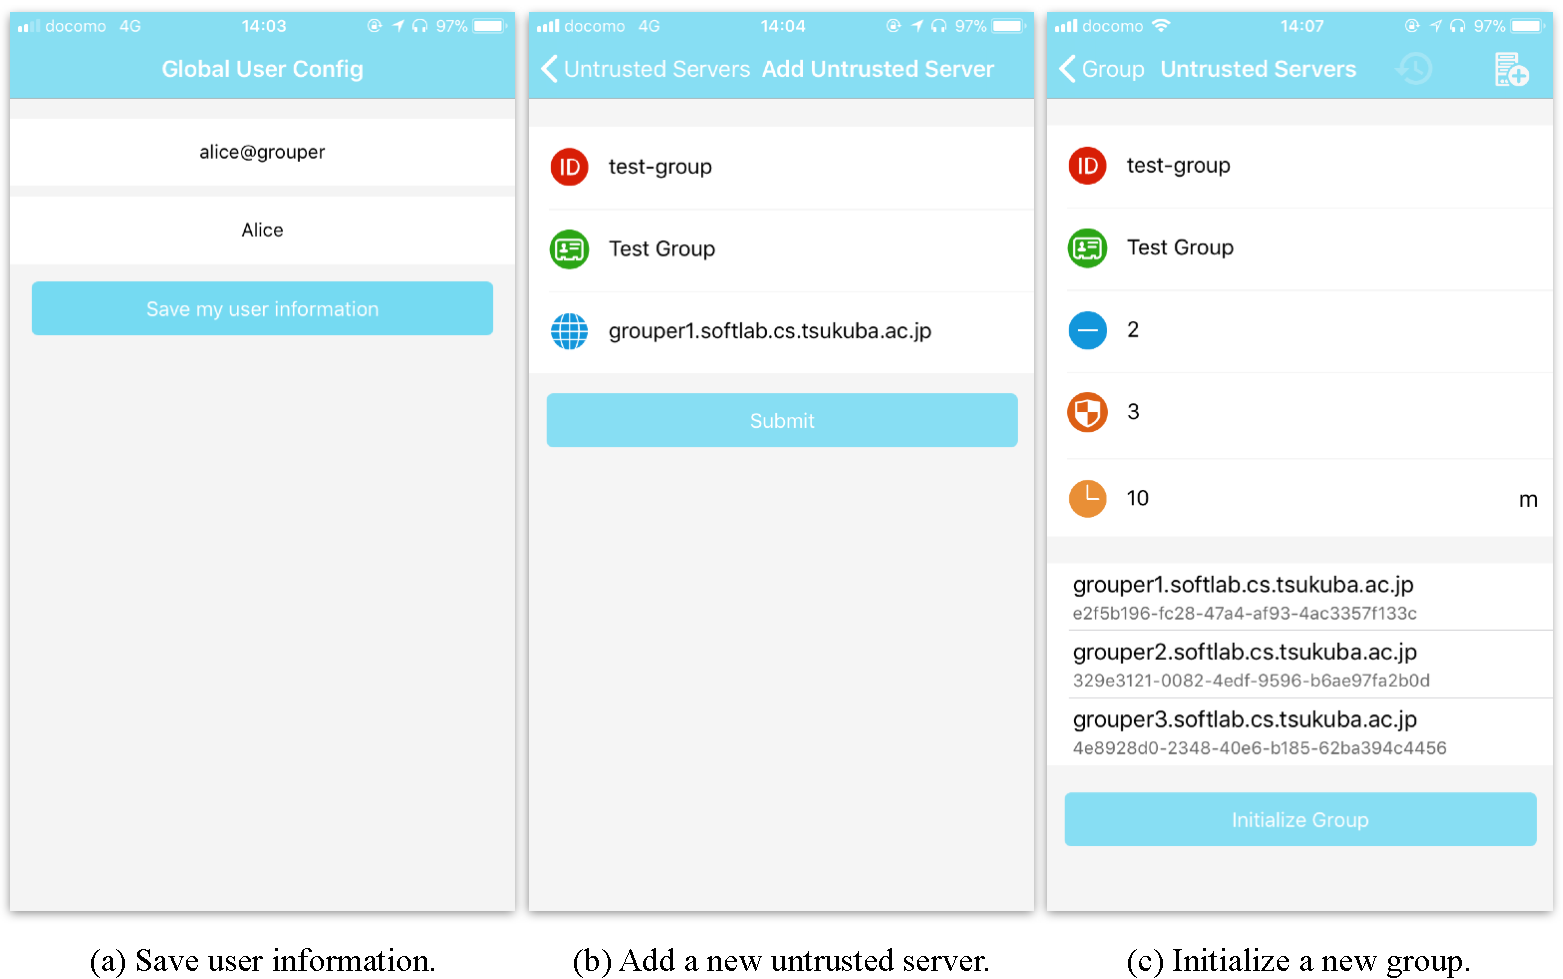
\includegraphics[scale=0.58]{group_manager_screenshot}
	\caption{Add an untrusted server and create a new group.}
	\label{fig:group_manager_screenshot}
\end{figure}

To simplify the application development using Grouper on the iOS platform, we provided the software development kit (SDK) on Grouper's client framework for the iOS platform.
Concretely, we encapsulate the methods about group creation and member invitation introduced above and create the GUI as shown in Figure \ref{fig:group_manager_screenshot}.
Figure \ref{fig:group_manager_screenshot} (a) shows the screenshot of saving user information using the  $- (void)saveCurrentUserWithEmail:name:$ method.
Figure \ref{fig:group_manager_screenshot} (b) shows the screenshot of adding a new untrusted server using the  $- (void)addNewServer:withGroupName:andGroupId:completion:$ method.
Figure \ref{fig:group_manager_screenshot} (c) shows the screenshot of initializing a new group using the  $- (void)initializeGroup:safeServersCount:interval:withCompletion:$ method.
With the iOS SDK of Grouper, a developer does not need to implement the group management by themselves using the methods in GroupManager. 

\subsection{Release and Installation}

We use CocoaPods\cite{cocoapods}, a dependency manager for Swift and Objective-C Cocoa projects, to release the client framework of Grouper.
With CocoaPods, the developer can add the dependency of Grouper to his / her applications easily.
To install the Grouper framework, a developer needs to add a file name Podfile including the following content.

\begin{lstlisting}[frame=none language=Ruby] 
use_frameworks!

target 'YourProjectName' do
    pod 'Grouper', '~>2.1'
end
\end{lstlisting}

The developer sets his / her project name as the target and the version of Grouper.
Then, he / she runs the following script in the terminal to install the Grouper framework.
CocoaPods dependency manager should be install before installing the Grouper framework.

\begin{lstlisting}[frame=none language=shell] 
# Run this script if CocoaPods is not been installed.
sudo gem install cocoapods

# Install Grouper with CocoaPods
cd [YourProject]
pod install
\end{lstlisting}

\section{Application} \label{section:application}

Using the Grouper framework, we have developed the following applications. 

\begin{itemize}
	\setlength{\itemsep}{1pt}
	\setlength{\parskip}{0pt}
	\setlength{\parsep}{0pt}
	\item \textbf{Account Book.} An iOS application in Objective-C, that records the income and expenditure of a group.
	\item \textbf{Test.} A benchmark iOS application in Swift, that tests the performance of Grouper.
\end{itemize}

We will introduce how to extend a standalone application into a data sharing application using Grouper.
In this section, we will show how we use Grouper to develop the demo application Account Book.
We have introduced the basic functions of Account Book in Section 4.1.
The standalone application of Account Book can record the income and expenditure of a small group by group members.
Without data sharing, records by a group member cannot be shared with other members.
To extend the stand alone application, we need follow the five steps as the following.

\subsection{Initialization of Grouper}

At first, we invoke the $grouper.setup()$ method introduced in Table \ref{table:grouper_api} to initialize Grouper in the method $- (BOOL)application: didFinishLaunchingWithOptions:$ of the AppDelegate at first.
Figure \ref{fig:initialize_grouper} shows how we initialize our Grouper framework in the Account Book application.
We invoke the class method $Grouper.sharedInstance$ to get the singleton of the Grouper framework in line 1.
Because our framework supports the GUI if iOS, we can provide the storyboard instance to Grouper to use the GUI for creating a new group or joining an existing group provided by Grouper.
For this reason, we get the storyboard instance in line 2.
In line 3, we invoke the initialization method to initialize Grouper.

\begin{figure}
\begin{lstlisting}[frame=none language=Objective-C] 
grouper = [Grouper sharedInstance];
UIStoryboard *storyboard = [UIStoryboard storyboardWithName:@"Main" bundle:nil];
[grouper setupWithAppId:@"accountbook"
entities:[NSArray arrayWithObjects:@"Classification", @"Account", @"Shop", @"Photo", @"Template", @"Record", nil]
dataStack:[self dataStack]
mainStoryboard:storyboard];
\end{lstlisting}
\caption{Initialize Grouper in the Account Book application.}
\label{fig:initialize_grouper}
\end{figure}

We have emphasized the order of the parameter entities in Table \ref{table:grouper_api}.
The reference relationships among entities Classification, Account, Shop, Photo, Template and Record are as following.

\begin{itemize}[leftmargin=7mm]
	\setlength{\itemsep}{1pt}
	\setlength{\parskip}{0pt}
	\setlength{\parsep}{0pt}
	\item \textbf{Record:}
	$Classification \gets Record, Account \gets Record, Shop \gets Record, Photo \gets Record$
	\item \textbf{Template:} 
	$Classification \gets Template, Account \gets Template, Shop \gets Template$
\end{itemize}

We can see the array in the code above following the principle introduced in Table \ref{table:grouper_api}.
For each entity, if it is referenced by an other entity, it is in front of the entity.
After initializing the Grouper framework in the Account Book application, we can invoke other methods in Table \ref{table:grouper_api}.

\subsection{Object Creation and Updating}

\begin{figure}[t]
	\centering
	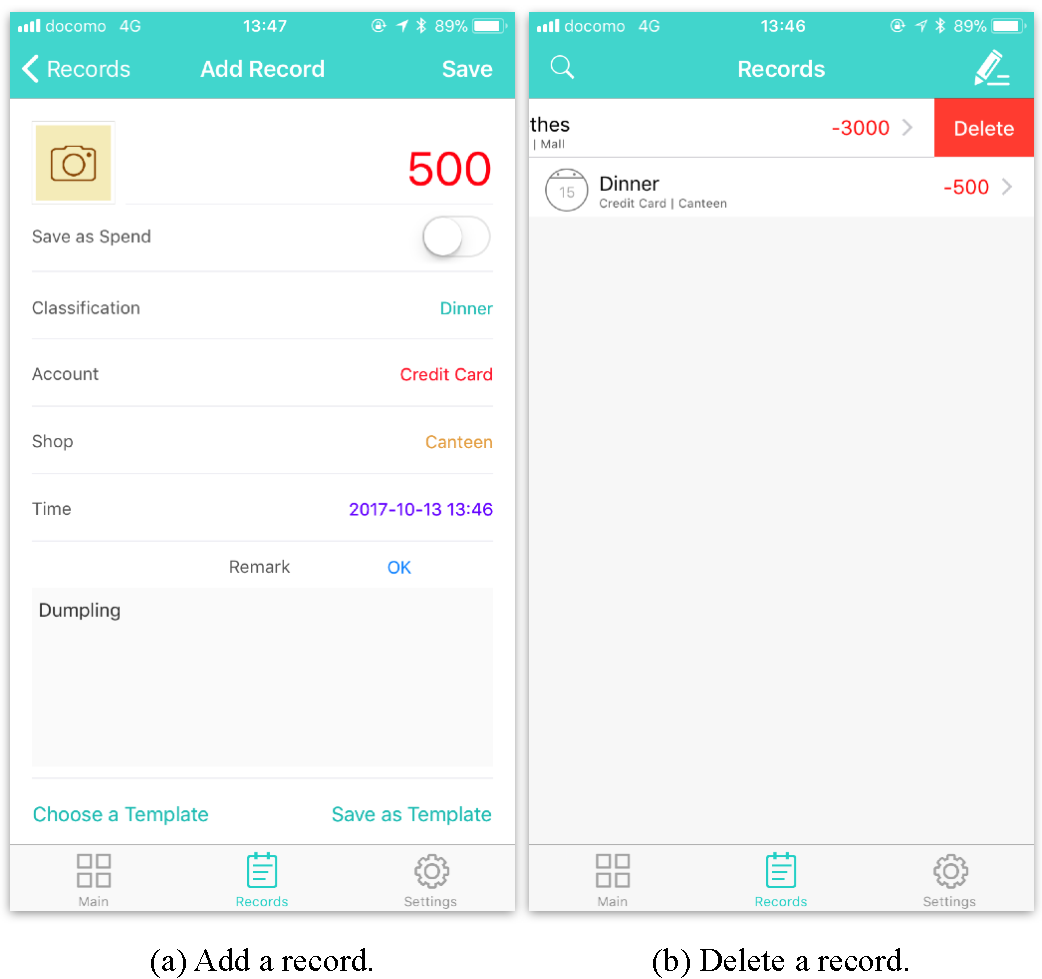
\includegraphics[scale=0.8]{account_book}
	\caption{Add and delete a record in the Account Book demo application.}
	\label{fig:add_delete_record}
\end{figure}

Figure \ref{fig:add_delete_record}(a) shows the screenshot of adding a record in Account Book. 
A user uses Account Book to add income and expenditure records that include the classifications, accounts, shops, times and remarks. 
When the user click the save button, Account Book saves the record into the local persistent store at first.
The stand alone application contains the line 2 to line 8.
To share this record with other group members, we invokes the $grouper.sender.update()$ method of Grouper to share this record with other group members after saving in the local persistent store in line 11.

\begin{figure}
\begin{lstlisting}[frame=none language=Objective-C] 
// Save record to app local persistent store.
Record *record = [dao.recordDao saveWithMoney:money
                       remark:_remarkTextView.text
                       time:_selectedTime
                       classification:_selectedClassification
                       account:_selectedAccount
                       shop:_selectedShop
                       photo:photo];

// Invoke update method in sender to send an update message.
[grouper.sender update:record];
\end{lstlisting}
\caption{Create a new record and send an update message.}
\label{fig:create_record}
\end{figure}

After invoking the method $grouper.sender.updated()$, this record will be divided to several shares and uploaded to multiple untrusted servers.
This method is also suitable for record updating.
Note that after invoking this method, data of the object has only been uploaded to multiple untrusted servers.
Grouper does not ensure that other grouper members can synchronize this object successfully.

\subsection{Object Deletion}

Figure \ref{fig:add_delete_record}(b) shows the screenshoot of deleting a record in Account Book. 
A user swipes a cell from right to left to delete a record from the record list.
In the stand alone application, we only delete this record in the local persistent store when the user click the delete button.
To delete this record on the devices of other group members, we invoke the $grouper.sender.delete(object)$ method of Grouper in line 4.

\begin{figure}
\begin{lstlisting}[frame=none language=Objective-C] 
Record *record = [records objectAtIndex:indexPath.row];
if (editingStyle == UITableViewCellEditingStyleDelete) {
    // Delete the record in the local persistent store and other devies.
    [grouper.sender delete:record];
    // Update user interface.
    [records removeObjectAtIndex:indexPath.row];
    [tableView deleteRowsAtIndexPaths:[NSArray arrayWithObject:indexPath] withRowAnimation:YES];
}
\end{lstlisting}
\caption{Delete a record and send a delete message.}
\label{fig:delete_record}
\end{figure}

By invoking the method $sender.delete()$, the record in the local persistent store will be deleted at first, so we need not to delete it on the local device before invoking this method like the method $sender.update()$.

\subsection{Synchronization from Untrusted Servers}

Grouper provide the method $grouper.receiver.receive()$ to synchronize messages from untrusted servers.
Developers can decide when and how to synchronize messages that contains the updated or deleted objects by themselves.
For example, we provide the following two ways in Account Book for users to synchronize messages.

\begin{itemize}[leftmargin=7mm]
	\setlength{\itemsep}{1pt}
	\setlength{\parskip}{0pt}
	\setlength{\parsep}{0pt}
	\item \textbf{Manually.}
	User can pull down the view as shown in Figure \ref{fig:receive_messages_send_confirm}(a) to synchronize messages.
	\item \textbf{Automatically when the application is launched.} 
	Account Book tries to synchronize messages automatically when it is launched.
\end{itemize}

We invoke the method $grouper.receiver.receive()$ to receive and synchronize messages, and update user interface or do other things in the callback block.
The parameter success in the block indicates the state of synchronization.
If the number of servers that a device can access is less than the threshold $k$ in the extend secret sharing scheme $f(k, n, s)$, the synchronization will be failed and parameter success will be false.

\begin{figure}
\begin{lstlisting}[frame=none language=Objective-C] 
[grouper.receiver receiveWithCompletion:^(int success, Processing *processing) {
    long now = (long)[[NSDate date] timeIntervalSince1970];
    if (now - grouper.group.defaults.controlMessageSendTime > grouper.group.defaults.interval * 60) {
        [grouper.sender confirm];
        // Update the last time to send a confirm message.
        grouper.group.defaults.controlMessageSendTime = now;
    }
}];
\end{lstlisting}
\caption{Receive messages from untrusted server and send a confirm message.}
\label{fig:receive_with_completion}
\end{figure}

\begin{figure}[t]
	\centering
	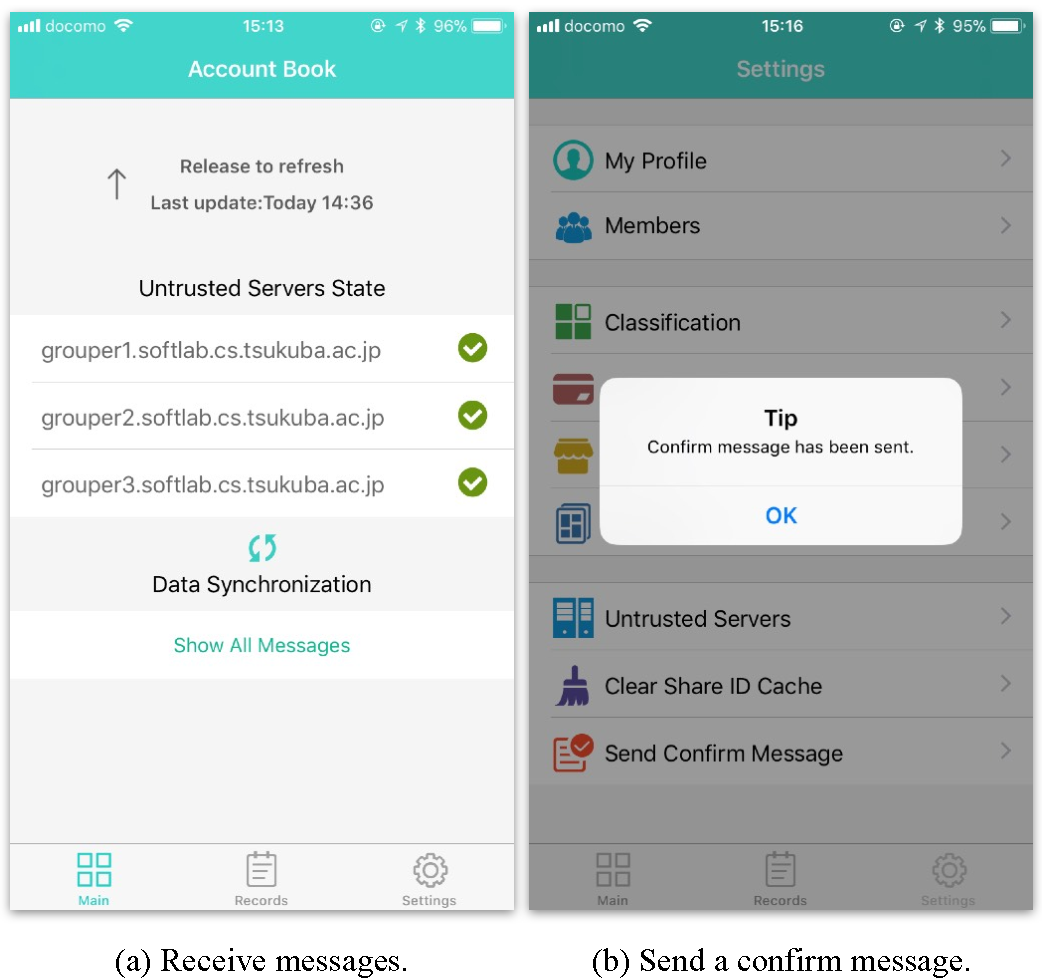
\includegraphics[scale=0.8]{receive_confirm}
	\caption{Receive messages and send a confirm message in the Account Book demo application.}
	\label{fig:receive_messages_send_confirm}
\end{figure}

\subsection{Sending Confirm Message}

We have introduced that method $grouper.confirm()$ is invoked periodically or when the device becomes online in Section \ref{section:grouper_message_protocol}.
In the Account Book application, we provide the following two ways to send a confirm message.

\begin{itemize}[leftmargin=7mm]
	\setlength{\itemsep}{1pt}
	\setlength{\parskip}{0pt}
	\setlength{\parsep}{0pt}
	\item \textbf{Manually.}
	User can send a confirm message manually in the Setting table view as shown in Figure \ref{fig:receive_messages_send_confirm}(b).
	\item \textbf{After receiving messages.}
	As described from line 2 to line 7 in Figure \ref{fig:receive_msg_send_confirm}, if Account Book receives messages from untrusted servers successfully, Account Book will check the last time to send the confirm message.
	If the time difference between now and the last time is longer than the TTL defined by user, Account Book will send a confirm message.

\end{itemize}

\chapter{Evaluation} \label{chapter:evaluation}

This chapter discusses the development efforts of applications using Grouper for developing mobile applications, as well as its performance.

\section{Development Efforts} \label{section:development_efforts}

\begin{table}
	\centering
	\caption{Application lines of code.}
	\label{table:loc}
	\begin{tabular}{lll}
		\toprule
		\textbf{Application} & \textbf{Account Book} & \textbf{Test} \\ 
		\midrule
		Platform & iOS & iOS \\ 
		Lanaguage & Objective-C & Swift \\ 
		Number of Entities & \multicolumn{1}{r}{5} & \multicolumn{1}{r}{1} \\ 
		Standalone Application LoC & \multicolumn{1}{r}{8076} & \multicolumn{1}{r}{621} \\ 
		Increased LoC &  \multicolumn{1}{r}{190} &  \multicolumn{1}{r}{18} \\ 
		\bottomrule
	\end{tabular}
\end{table}

We view the development efforts through two factors: the usability of the client API and the code size, in terms of the lines of code (LoC) the developer has to add after using Grouper. 
As described in Table \ref{table:grouper_api}, Grouper provides a simple client APIs for developers.
A developer can easily convert a standalone application to a data sharing application with our client APIs.

Section \ref{section:application} demonstrates the implementation of two applications.
Table \ref{table:loc} shows that developers can add data synchronization to these applications with Grouper by adding a small amount of code. 

The Grouper framework provides the synchronization as a pluggable module.
We use the Sync\cite{sync} framework.
It provides a consistency model where currently, the newest object wins in the synchronization plugin.
For example, if a record in the Account Book application has been modified by two users, the modification of one user will be lost.
Account Book maintains the newest modification and put it into persistent store.

If an application requires another consistency model, the developer has to implement the related synchronization plugin.
For example, if a developer wants to use eventual consistency, he/she can choose Ensembles\cite{ensembles}.
For this reason, if a developer wants to use another consistency model, he/she must add more lines of code to those in Table \ref{table:loc}.

Note that the synchronization frameworks must provide the interfaces as described in Table \ref{table:sync_plugin}.
For this reason, Grouper does not support iOS synchronization frameworks for iCloud or Dropbox.
For example, Grouper does not support Core Data with iCloud\cite{coredata} and TICoreDataSync\cite{ticoredatasyn} at this point.
These frameworks provide APIs for files whereas Grouper requires APIs for sending multicast messages.
If a developer want to use them, he/she has to add an additional layer that provides the methods in Table \ref{table:sync_plugin}.

\section{Performance} \label{section:performance}

\begin{table}[t]
	\centering
	\caption{Devices in the performance experiment.}
	\label{table:experiment_devices}
	\begin{tabular}{llll}
		\toprule
		\textbf{Device} & \textbf{CPU} & \textbf{RAM} & \textbf{OS} \\ 
		\midrule
		iPod touch 5th & A5 & 512MB & iOS 9.3.5 \\
		iPhone 4s & A5 & 512MB & iOS 9.3.5 \\
		Server 1 & Core i7-5820K & 32GB & Ubuntu 14.04.5 \\
		Server 2 & Core i7-5820K & 32GB & Ubuntu 14.04.5 \\
		Server 3 & Core i7-5820K & 32GB & Ubuntu 14.04.5 \\ 
		\bottomrule
	\end{tabular}
\end{table}

In this section, we show that mobile applications using the Grouper framework provide satisfactory performance for small groups of people.
Table \ref{table:experiment_devices} lists the hardware and software configuration of our experiment environment.
In our performance experiments, we used the benchmark application \emph{Test} to transfer data between the iPhone 4s and iPod touch 5th generation on a wireless LAN network (802.11n).
We installed 30 Web services on three different servers.
Each server ran a Tomcat server instance which hosted 10 Web services.

In our benchmark application, the size of an object was 323 bytes.
The object corresponded to an income or expenditure record of the Account Book application.
When the object was updated in a node, the Grouper API generated a normal message whose size was 656 bytes.

We performed an experiment to measure the processing time of object synchronization according to the number of updated objects.
In this experiment, we set the secret sharing scheme to ${f(2, 3, 3)}$.
We sent multiple messages from a device and received them in another device. 
Concretely, we sent multiple messages from the iPod to the iPhone for three times, and from the iPhone to the iPod for three times.
Then, we obtained the average value of the measured processing times.

\begin{figure}[t]
	\centering
	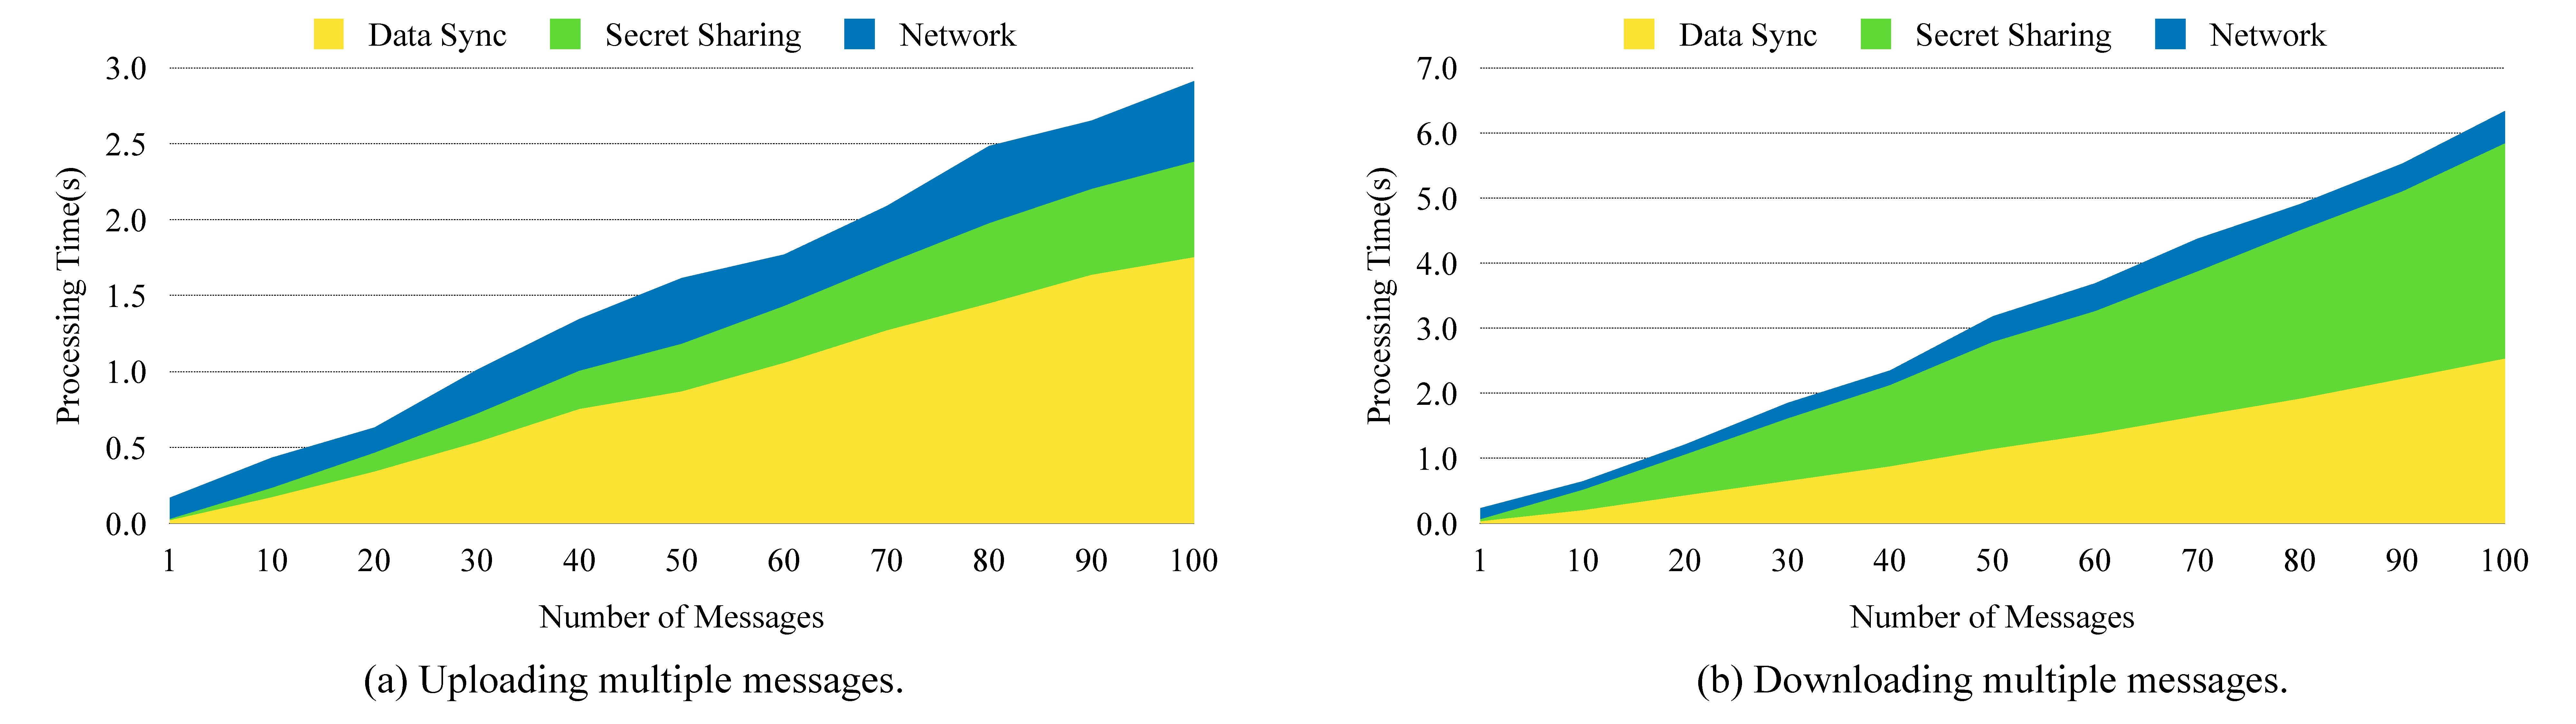
\includegraphics[scale=0.15]{multiple_messages}
	\caption{Processing time of uploading and downloading multiple messages.}
	\label{fig:processing_time_multiple_message}
\end{figure}

Figure \ref{fig:processing_time_multiple_message} shows the processing time of uploading and downloading multiple messages.
We divide the processing time into three parts: data synchronization, secret sharing, and networking.
As the number of messages increased, the data synchronization and secret sharing time increased linearly. 
The networking time increased slowly and sometimes decreased.
On the whole, the total processing time increased linearly.
Compared with uploading messages, downloading messages required more processing time.

Note that object synchronization is done as a background task, asynchronously.
When the Grouper framework is performing object synchronization, the user interface of a mobile application does not freezes.
Therefore, a user is not aware of the activity of data synchronization.

We performed an experiment to measure the processing time of object synchronization according to the parameters of the secret sharing scheme.
Specifically, we changed the parameter ${k}$ and ${n}$ of the secret sharing scheme and measured the processing time of uploading and downloading a single message.

\begin{figure}[t]
	\centering
	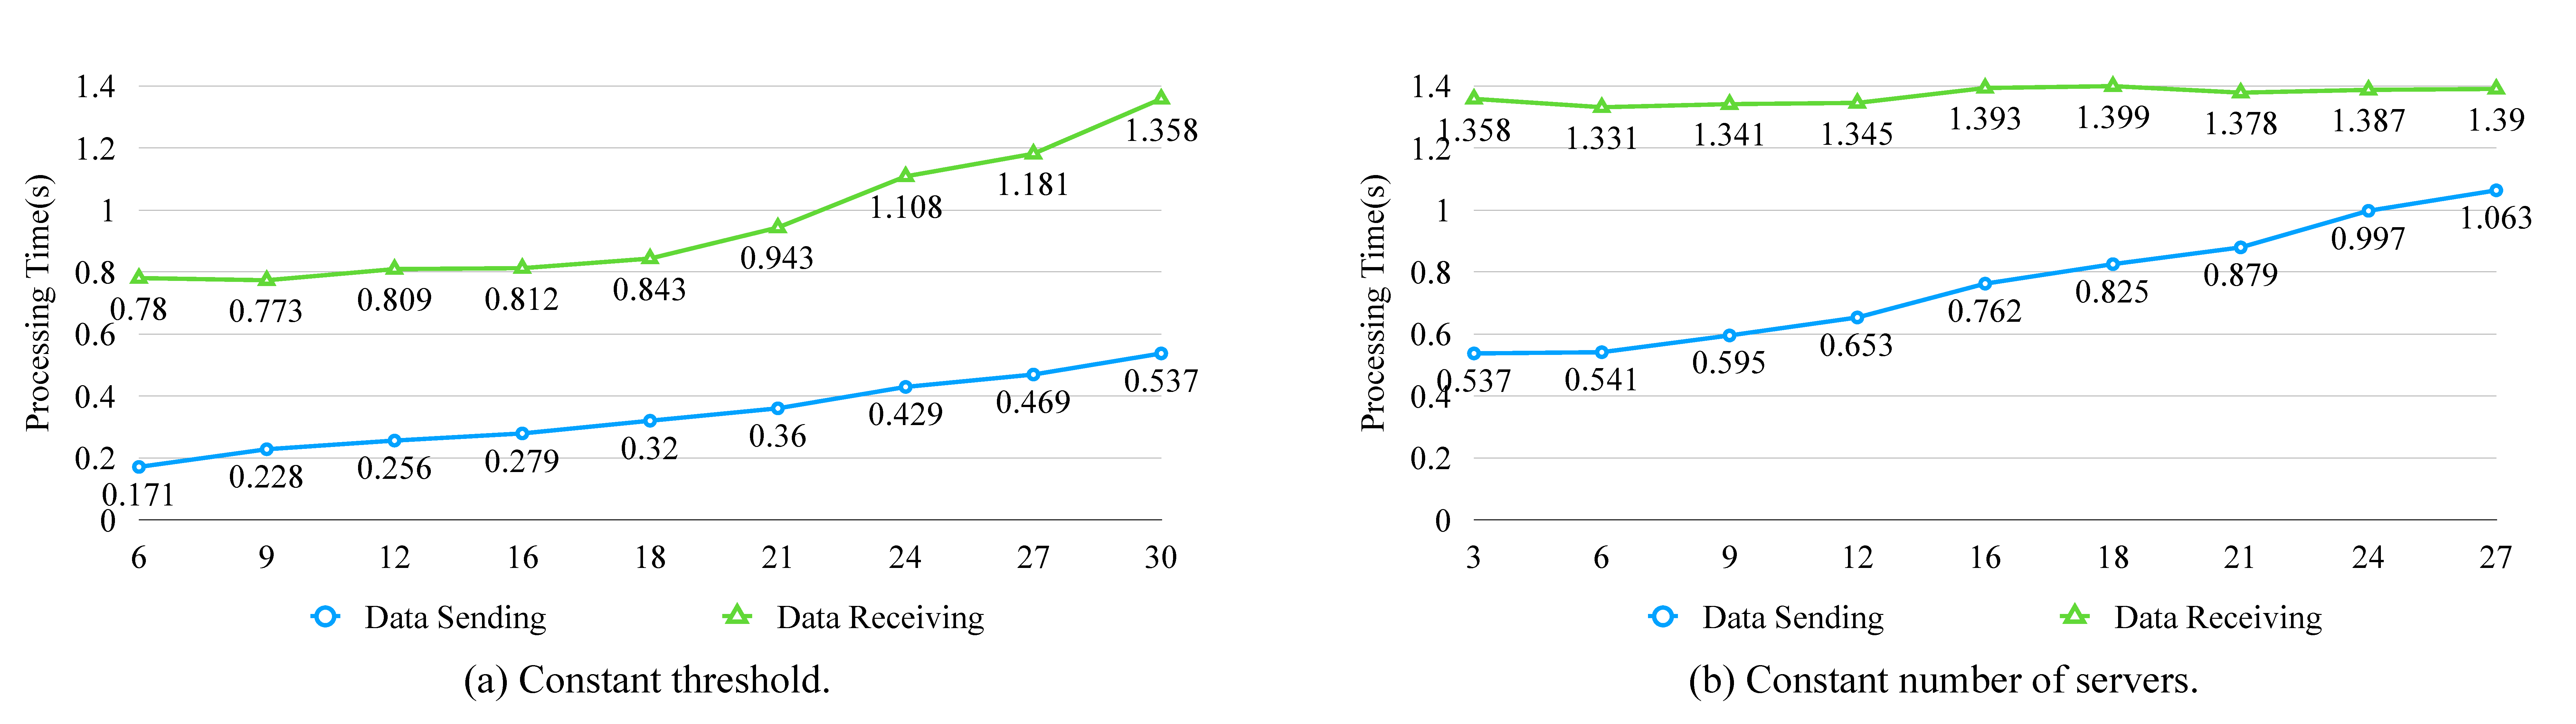
\includegraphics[scale=0.15]{constant_k_n}
	\caption{Processing time of uploading and downloading a single message with a constant ${k}$ or ${n}$.}
	\label{fig:processing_time_constant_k_n}
\end{figure}

Figure \ref{fig:processing_time_constant_k_n}(a) shows the relationship between processing time and the number of servers ${n}$, where ${k=3}$,  ${n = 6, 9, ... , 30}$ and $s = n$.
As $n$ increased, the processing time of uploading and downloading increased linearly. 
Figure \ref{fig:processing_time_constant_k_n}(b) shows the relationship between processing time and the threshold ${k}$, where ${n = s =30}$ and ${k = 3, 6, 9, ... , 27}$.
As $k$ increased, the processing time of uploading increased linearly and that of downloading did not change.

\section{Discussion on the Number of Messages} \label{section:discussion}

In this section, we discuss and the number of messages. 
We use the parameters in Table \ref{table:discussion_parameters}.

\begin{table}[t]
	\centering
	\caption{Parameters for discussing the number of messages.}
	\label{table:discussion_parameters}
	\begin{tabular}{ll}
		\toprule
		\textbf{Parameter} & \textbf{Explanation} \\ 
		\midrule
		$D$ & Number of devices. \\
		$T$ & Time to live (TTL). \\
		$F$ & Average number of offline devices during the TTL. \\
		$L$ & Average offline time. \\
		$Ui$ & 
		\begin{tabular}{@{}l@{}}
			Average number of updated/deleted messages in the device $i$ during\\ the TTL. 
		\end{tabular} \\ 
		$URi$ & 
		\begin{tabular}{@{}l@{}}
			Average number of updated/deleted messages by resend messages in\\ the device $i$ during the TTL.
		\end{tabular} \\ 
		$C$ & Average number of confirm messages in the device $i$ during the TTL. \\ 
		$U$ & Total number of updated and deleted objects during the TTL. \\ 
		$NUi$ & Number of uploads for device $i$ during the TTL. \\
		$NU$ & Total number of uploads during the TTL. \\
		$NDi$ & Number of downloads for device $i$ during the TTL. \\
		$ND$ & Total number of downloads during the TTL. \\ 
		\bottomrule
	\end{tabular}
\end{table}

First, we consider the situation in which all devices are online ($F=0$).
In this situation, the number of uploads for the device $i$ are:

\begin{equation}
NUi = Ui + C
\label{equation:nui0}
\end{equation}

Total number of uploads $NU$ is the sum of $NUi$.

\begin{equation}
NU = \sum_{i = 1}^{D} NUi = U + C \cdot D
\label{equation:nu0}
\end{equation}

A device does not download the messages that is has uploaded.
To simplify these equations, we assume that the device downloads those messages as well.
Thus, the number of downloads for device $i$, $NDi$, is the equal to the total number of uploads $NU$.

\begin{equation}
NDi = NU = U + C \cdot D
\label{equation:ndi0}
\end{equation}

The total number of downloads $ND$ is the sum of $NDi$.

\begin{equation}
ND = \sum_{i = 1}^{D} NDi = NU \cdot D =  (U + C \cdot D) \cdot D
\label{equation:nd0}
\end{equation}

Since the current cloud servers scale well according to the number of devices and and messages, we discuss $NUi$ and $UDi$ in this section.
Equation \ref{equation:nui0} shows that for the device $i$ during the TTL, the order of uploading is $O(U)$.
Euqation \ref{equation:ndi0} shows that the order of downloading is $O(U+D)$.
As the number of updated and deleted objects increases, the total numbers of uploads and downloads increases linearly.
As the number of devices increases, the number of confirm messages increases linearly.

Next, we consider the situation in which there are offline devices in a group ($F \neq 0$).
In this situation, offline devices send resend messages when they become online and the devices that have the updated objects will resend the update messages to the offline devices.
To simplify these equations, we assume that all offline devices receive the updated messages after they send resend messages.
For the device $i$, the number of those update messages by the resend message, $URi$, is

\begin{equation}
URi = Ui \cdot \frac{L}{T} \cdot F
\label{equation:uri}
\end{equation}

Compared to the situation that $F=0$, in this situation, the number of uploads for the device $i$ includes $URi$.
Thus, we obtain $NUi$, $NU$, $NDi$ and $ND$ where $F \neq 0$.

\begin{equation}
NUi = Ui + C + Ui \cdot \frac{L}{T} \cdot F = Ui \cdot (1 + \frac{L}{T} \cdot F) + C
\label{equation:nui}
\end{equation}

\begin{equation}
NU = \sum_{i = 1}^{D} NUi = U \cdot (1 + \frac{L}{T} \cdot F) + C \cdot D
\label{equation:nu}
\end{equation}

\begin{equation}
NDi = NU = U \cdot (1 + \frac{L}{T} \cdot F) + C \cdot D
\label{equation:ndi}
\end{equation}

Equations \ref{equation:nui} and \ref{equation:ndi} show that for the device $i$ during the TTL, the order of uploading is $O(U \cdot \frac{L}{T} \cdot F + C)$, and the order of downloading is $O(U \cdot \frac{L}{T} \cdot F + C \cdot D)$.
As the numbers of updated and deleted objects, the average number of offline devices during the TTL, and the average online time increase, the number of uploads and downloads for a single device increases linearly.

If we use a longer $T$, the numbers of messages, $NUi$ and $NDi$, become smaller.
However, this makes it easier for attackers to attack untrusted servers.

Finally, we consider the following two cases with concrete parameters.
In the last two cases, there are ten users in a small group and everyone has a device.
We set the TTL to one day and a hundred of normal messages are created by the ten users in the group during the TTL.
In addition, a device send only one confirm message during the TTL.

\begin{itemize}[leftmargin=7mm]
	\setlength{\itemsep}{1pt}
	\setlength{\parskip}{0pt}
	\setlength{\parsep}{0pt}
	\item \textbf{Case 1: $D = 10,\ T = 1 \ day,\ Ui = 100,\ C = 1,\ F = 0$.}
	
	In this case, there are no offline users in the group.
	Each device uploads 101 messages and downloads 1010 messages during the TTL.
	\item \textbf{Case 2: $D = 10,\ T = 1 \ day,\ L = 1 \  day,\ Ui = 100,\ C = 1,\ F = 2$.} 
	
	In this case, there are two offline users in the group and the average offline time is one day.
	Each device uploads 301 messages and downloads 3010 messages during the TTL.
\end{itemize}

\section{Scalability of Grouper} \label{section:grouper_scalability}

From section \ref{section:development_efforts} to \ref{section:discussion}, we can conclude that Grouper is able to support a group with a hundred of members, and does not influence user experience of an application.

\chapter{Conclusion} \label{chapter:conclusion}

This thesis concentrates on developing mobile application on top of a self-destruction system with data recovery.
For this goal, we developed Grouper, a framework using a secret sharing scheme and multiple untrusted servers, to implement light-weight information sharing in mobile applications.

Chapter \ref{chapter:introduction} points out the problems of the mobile applications using the central servers to store user data.
Although some data self-destruction systems tries to solve this problem by encrypting user data and keeping it in the servers temporarily, they do not support data recovery after deleting data.
Therefore, we developed the Grouper framework based on the theory of self-destruction system and supported data recovery in Grouper.

Chapter \ref{chapter:related_work} introduces related work.
First, we introduce Data self-destruction systems including Vanish, SafeVanish, SeDas and CloudSky.
They are suitable for developing news systems without data recovery.
Compared to conventional self-destruction systems, Grouper provides the reliable synchronization and allows mobile devices to synchronize data with other devices after untrusted severs remove the data.
Second, we introduces data encryption systems including Mylar, Sweets, DepSky and SPORC.
These systems usually need key generation and distribution.
Compared to pure data encryption approaches, Grouper improves dependability by using multiple untrusted servers and an extended secret sharing scheme $f(k, n, s)$.

Chapter \ref{chapter:threat_model} proposes the threat model of Grouper.
In an target application using Grouper, users can create a group and share objects safely via multiple untrusted servers.
Grouper provides two main functions: reliable data synchronization and group management.
To develop the target applications, we proposes four assumptions for Grouper including servers without actively attacking, safe data transportation, trusted group members, independent server providers.

Chapter \ref{chapter:design} presents the design of Grouper.
Grouper includes a client framework and a Web service.
Concretely, Grouper consists of the Grouper API layer, synchronization plugin, messaging layer, data protection layer, and untrusted servers.
The Grouper API layer provides methods for sharing data among devices of a group.
The synchronization plugin helps Grouper to synchronize data into the persistent store.
Based on the basic reliable multicast technique, the messaging layers ensures reliable messages delivery using a special type of message that includes active sequence numbers.
The data protection layer uses the extended secret sharing scheme $f(k ,n, s)$ to protect the user data.
To manage a group, Grouper provides two functions including group creation and member invitation.

Chapter \ref{chapter:implementation} involves the implementation details of Grouper using the Java language and the Objective-C language.
We have implemented the Web service in the Java language and Grouper's client framework in the Objective-C language.
The Web service running on the Tomcat server provides RESTful API for the client framework. 
The managers including SenderManager, ReceiverManager and GrouperManager in the client framework invokes the RESTful API to send / receive messages and manage a group.
Grouper's client framework can be installed with the CocoaPods dependency manager easily.
In addition, we have developed applications, \emph{Account Book} and \emph{Test}, using Grouper.
We introduces how to develop Account Book using Grouper including framework initialization, object creation / updating / deletion, and synchronization.

Chapter \ref{chapter:evaluation} gives a evaluation of Grouper and discusses its scalability.
The development of these applications demonstrate that Grouper requires little development effort to convert an standalone application into a data sharing application.
We also evaluated the performance of Grouper using our benchmark application.
The results shows that using Grouper in an application does not influence user experience.

In the future, we would like to support additional platforms, including Android.
We also have a plan to use file-oriented APIs for exchanging messages among devices.

\chapter*{Acknowledgements}
\addcontentsline{toc}{chapter}{\numberline{}Acknowledgements}

The author would like to express my gratitude to my supervisor Professor Yasushi Shinjo for the useful comments, remarks and engagement through the learning process of this master thesis.

The author would like to thank Elvis Nun{\~e}z for helping us to fix some Objective-C related issues of the Sync framework, and Bernard Paulus for fixing a bug of c-SSS, an implementation of the secret sharing scheme.

The author would like to thank Professor Au Thien Wan from Unniversiti Teknologi, Brunei, for giving some suggestions about future work, and Associate Professor Dan Li from Northeast Forestry University, China, for giving some suggestions about design of the framework.
The author would like to thank Yifan Li for giving some suggestions about English grammar.

This work was partially supported by JSPS KAKENHI Grant Number 16H02805.

\newpage

%% Bibliography
\addcontentsline{toc}{chapter}{\numberline{}Bibliography}
\renewcommand{\bibname}{Bibliography}
% use bibtex
%\bibliographystyle{unsrt}
%\bibliography{samplebib}
%% [compile] bibtex sample-en; platex sample-en; platex sample-en;

% describe bib entries in the file
\bibliographystyle{unsrt}
\bibliography{ref} 


\end{document}
